\chapter[CVS Pose Measurement Error]{Computer Vision System Pose Measurement Error}
\label{chap4}

\section{Introduction}

The main objective of this project is to determine the pose estimation accuracy of a quadcopter's on-board sensor suite. The pose estimation must be performed in the outdoors to provide the quadcopter access to its GPS readings, which is important data for an outdoor quadcopter since it provides absolute position data which can be used to offset the sensor drift introduced by integrating other sensor data. To this end, a computer vision pose measurement system (CVS) which extracts six-dimensional pose data from a calibration object in the system's view, was designed and implemented. However, before the CVS could be used to make pose measurements, its measurement accuracy was first determined. 

In Chapter~\ref{chap3} it was found that the pose measurement error of the CVS displays high interdimensional dependence, as demonstrated by the covariance matrix of the CVS's measurement error data in Equation~\ref{eq:covariance-matrix} and the contour plots in Figure~\ref{fig:err-contour}. This means that the CVS's pose measurements and corresponding measurement errors are constantly varying according to the relative pose between the calibration board and the CVS's camera. Also, despite using the RANSAC algorithm to filter out outlier data points, the CVS's measurement data is still fairly noisy, particularly in the orientation dimensions.

In the context of this project it is important to know what the accuracy of a pose measurement sample is. This makes it necessary to be able to determine the measurement error of any arbitrary pose measurement sample recorded by the CVS.\@ It was decided that a machine learning method will be employed to accomplish this. Machine learning is where a computer model is trained to recognise patterns within a set of input data and output information on the patterns which are of interest to the model's designer. 

This chapter sets out to explain the process behind making a machine learning model that can estimate, with reasonable accuracy, what the CVS's pose measurement error for any arbitrary input measurement vector would be. This chapter has been presented at the SolarPACES 2015 conference in Cape Town and a conference proceedings article has been accepted, pending publication~\citep{lock2015}. 

The chapter starts with some background information on model selection, design and training. The validation phase of the trained model is then discussed and the accuracy of the final model is presented, followed by a brief discussion on the resulting model. 

\section{Model Design}

This section discusses the design aspects of the machine learning model used for this project. It begins by giving some background information on the processes involved in designing such a model, including model type selection, training and validation. These aspects are discussed in more detail here.  

\subsection{Background}

Designing a machine learning model can be performed in three basic steps. These steps are:

\begin{enumerate}
  \item Select machine learning model type.
  \item Train the model.
  \item Validate the trained model's accuracy. 
\end{enumerate}

First, the model type is selected. As stated previously, the CVS's pose measurement data is fairly complex, interdimensionally dependant and high dimensional. A neural network was therefore selected as a machine learning model basis. It has previously been shown by~\cite{tu1996advantages} that neural networks excel at handling complicated data and detecting and extracting complex, non-linear relationships within the input data. Furthermore, the radial basis function neural network (RBFNN) was selected as the network topology. RBFNN's provide superior results when compared to traditional feed-forward networks when noisy data sets are used, as shown by~\cite{xie2011comparison}. The data is not time dependant, making the recurrent neural network topology unnecessarily complex and costly for this application. An RBFNN is described by the relation given by Equation~\ref{eq:chap2-rbf} and is repeated again in Equation~\ref{eq:chap4-rbf}.

\begin{equation}
  \label{eq:chap4-rbf}
  f(\bm{x}_i) = \sum\limits_{j = 1}^{M}\lambda_j \phi(|| \bm{x}_i - \bm{x}_j ||)
\end{equation}
Here, $\phi$ is a function of the Euclidean distance between the radial basis centres, $\bm{x}_j$, and the sample points, $\bm{x}_i$.

Next, model training takes place where the network is trained with a supervised learning scheme, such as the backrpopagation procedure, to take an input and adjust its internal weights in such a way that the input data is best translated to the desired output. In this case, the network input was the six-dimensional pose vector produced by the CVS and the network output was the corresponding measurement error of the input pose vectors.  

Finally, to test and validate the accuracy of the trained model, it is tested with another set of input pose data of which the measurement error is already known. This data set can then be used to select and refine the training parameters of the network model. 

The design process is iterative, where steps 2 and 3, and perhaps 1, can be repeated until a network which outputs satisfactory results is produced. 

\subsection{Network Training}

Training a machine learning model is perhaps the most crucial aspect of the model design phase. Here, the nodes of the RBFNN are initialised and assigned a weighting factor. The weightings are then adjusted and optimised through a supervised training method called backprogagation, demonstrated in Figure~\ref{fig:chap4-backprogagation}. The number of radial bases can also be optimised to produce the best results, but in this case it was preselected. 

\begin{figure}
  \centering
  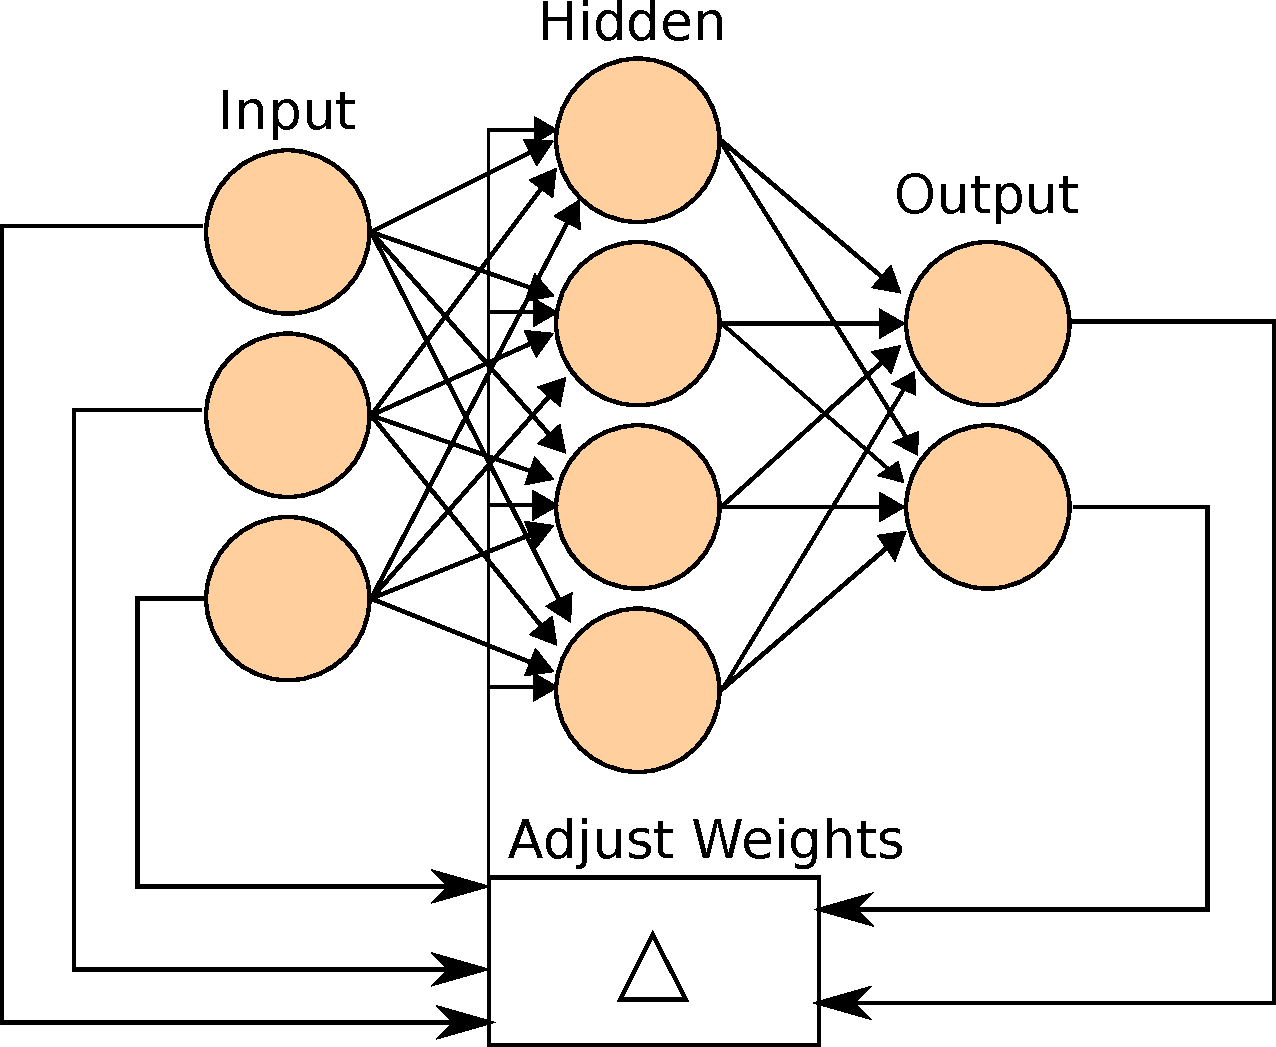
\includegraphics[width=0.5\textwidth]{figures/chapter4/backpropagation}
  \caption[A neural network implementing the backpropagation procedure.]{A figure of a neural network implementing the backpropagation procedure. Adapted from~\cite{ann-wiki-pic}.}
\label{fig:chap4-backprogagation}
\end{figure}

Backpropagation works as follows. The hidden nodes are given an initial weighting factor. The input training data is then fed to the network and its output is compared to the training set's output data. Based on this difference, the hidden nodes' weightings are adjusted in an attempt to minimise the difference. Then, the input data is fed to the adjusted network again and its new output is compared to the output training data, where the weights are adjusted again. This process is repeated until the mean square error (MSE) of the output's deviation from the training data falls below a set threshold or converges to zero. 

Factors that will affect the network's accuracy are the number of nodes, or radial bases, in the hidden layer as well as the strictness of fit that the designer selects. The number of hidden nodes is a measure of the complexity of the data the network can process and also reflects own complexity. However, when too many nodes are initialised there is a significant risk that the network will capture and attempt to model the noise and outlier data in a data set, instead of only characterising the underlying relationships between the input and output. This phenomenon is known as overfitting and can be observed when a network with a very small training MSE is exposed to new input data and the MSE is a few orders of magnitude larger than for the training data. Therefore, the validation phase is also an important aspect of network training to ensure that overfitting does not take place. 

The strictness of fit measure determines to what extent the network will attempt to fit itself to the training data. Selecting the right parameter is important, since neglecting to replicate the training data adequately defeats the purpose of training the network to fit the data in the first place. However, if this parameter is too strict, the network will attempt to model the outlier and noisy data points as well, which is undesirable. Therefore, a fine balance needs to be found for the strictness of fit and the number of hidden nodes to produce a satisfactory network.  

To train the network of this project, two sets of data was used; one set for training and another for validation. Both of these sets were taken from the data generated during the Vicon measurement test where the measurement accuracy of the CVS was determined. It includes both the pose data from the CVS and its corresponding measurement error. It was decided to use 300 training samples, giving 50 samples per dimension. The training data was selected to be uniformly distributed to place emphasis on the entire measurement spectrum. The uniformity of the data in each dimension was verified with the Chi-square ($\chi^2$) goodness-of-fit test, with the hypothesis being that the set is uniformly distributed. As a rule of thumb, if the P-value for the $\chi^2$ test falls below 5 \%, then the hypothesis is statistically insignificant and must therefore be rejected. The training data was selected such that the P-value did not fall below 45 \% for the data in each dimension. 

Since the pose vector contains different measurement units (degrees and metres), the input and output training data sets were normalised to a range of $[-1, 1]$. All subsequent inputs to and outputs from the network must be normalised and denormalised with the same values that the training data was normalised with. To further accommodate the inherent differences between position and orientation data, two RBFNNs were trained: one to estimate the position measurement error and another to estimate the orientation estimation error. Both networks still take 6 dimensional CVS pose measurements as inputs. Figure~\ref{fig:chap4-two-networks} shows the layout for the dual network configuration.

\begin{figure}
  \centering
  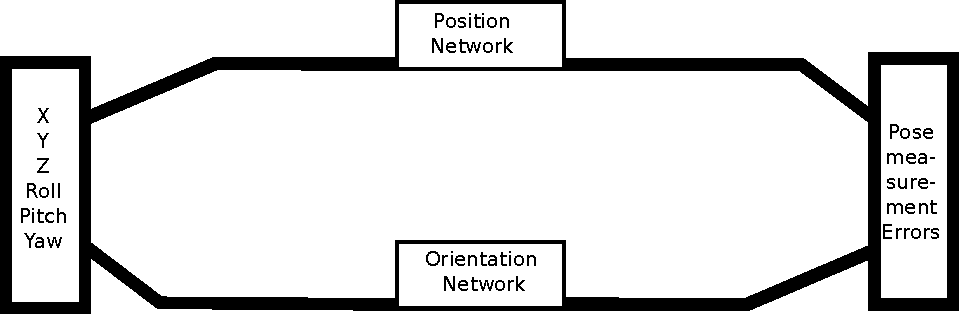
\includegraphics[width=\textwidth]{figures/chapter4/two_network}
  \caption{A figure showing the configuration for the dual RBFNN configuration.}
  \label{fig:chap4-two-networks}
\end{figure}

Matlab's\footnote{Matlab v8.4.0.150421 (R2014)} Neural Network toolbox\footnote{Neural Network Toolbox v8.2.1} was used to train the RBFNNs and get the output for subsequent input data. The function prototype is given by 

\begin{center}
  \verb|rbf = newrb(P,T,goal,spread,MN,DF)|.
\end{center}

Here, $P$ and $T$ are the input and output training data matrices. The \emph{goal} parameter is the error threshold for the training data and \emph{spread} is the strictness of fit parameter, while $\mathit{MN}$ and $\mathit{DF}$ define the maximum number of hidden nodes and dictate the amount of nodes to increase between each training iteration. Adjusting the \emph{spread} and $\mathit{MN}$ parameters are the primary ways of manipulating the networks and produce more accurate outputs. 

\subsection{Model Validation}

A model validation procedure was used to ensure that the RBFNNs were properly trained and that overfitting did not occur. The validation set comes from the same Vicon test that the training data was selected from. Another 300 randomly selected pose measurement samples were used for the validation data set. Given that the training data is uniformly distributed, the validation set fell within the training data limits. Figure~\ref{fig:chap4-scatter-tr-v} displays the scatter plots for the position and orientation vectors for the training and validation sets and shows that they indeed do overlap to a large degree. 

\begin{figure*}
  \centering
  \begin{subfigure}{\textwidth}
    \begin{subfigure}{0.48\textwidth}
      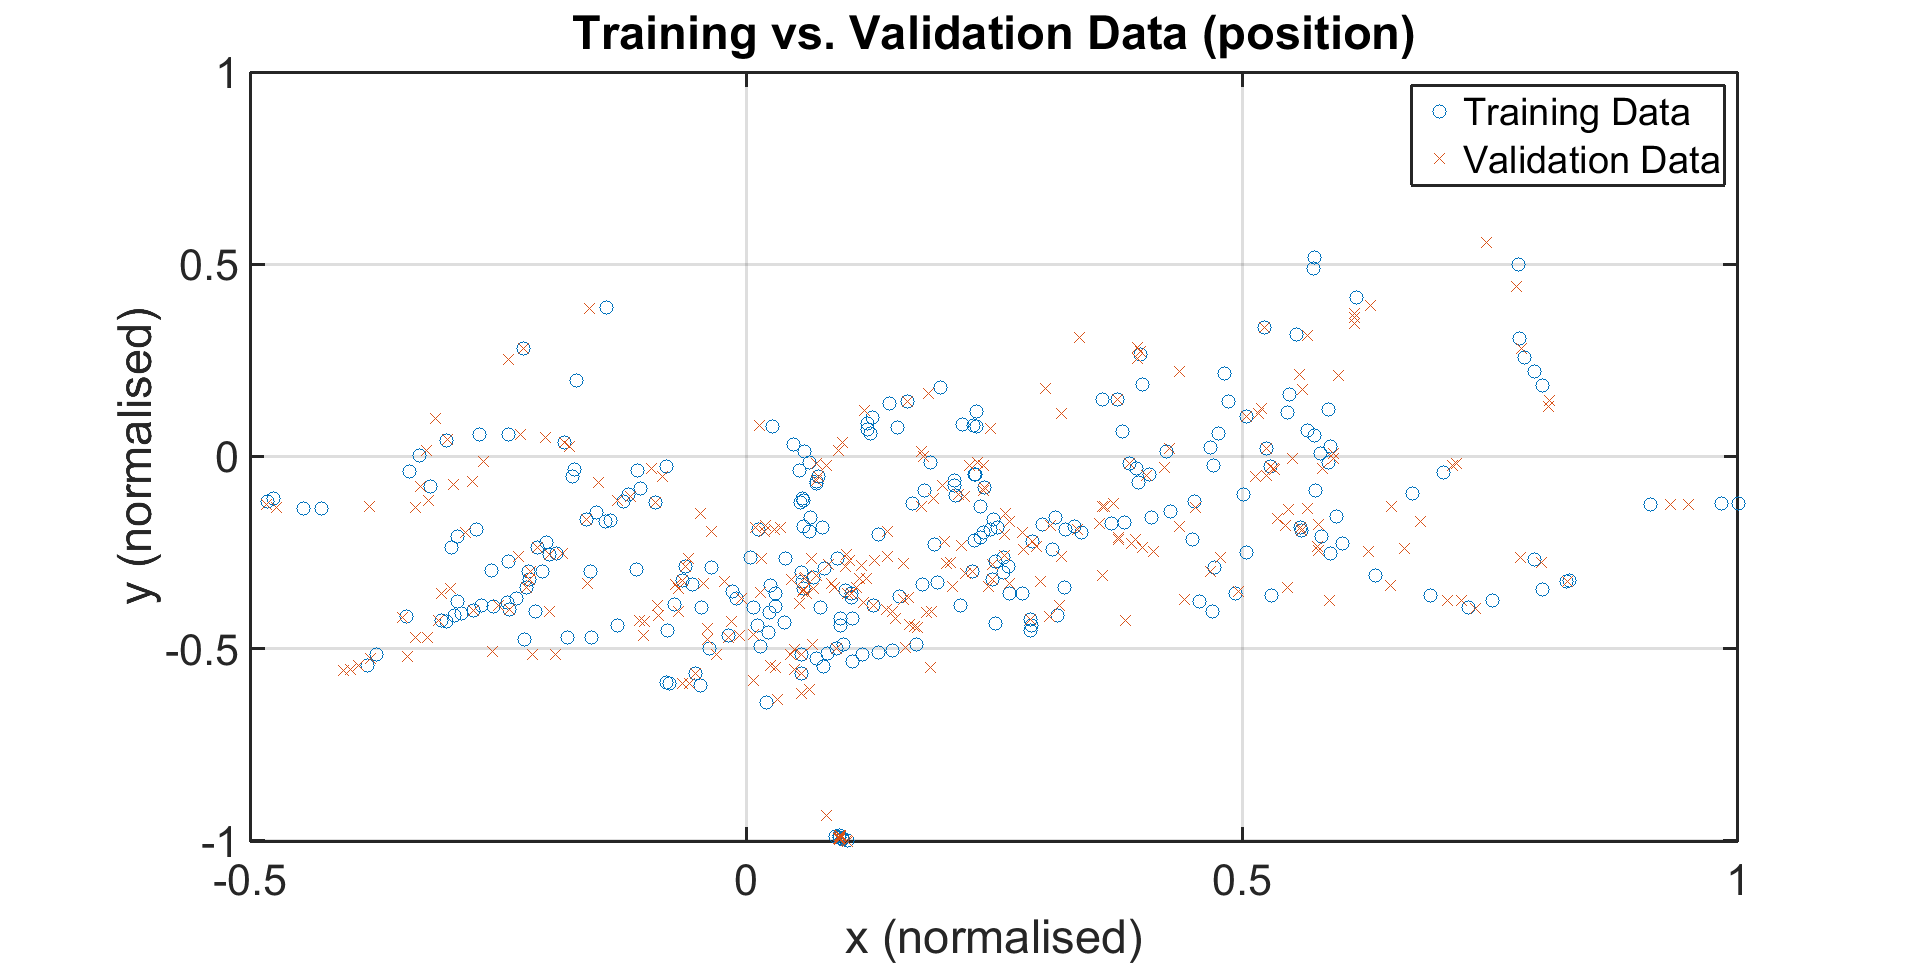
\includegraphics[clip, trim = 80 0 80 0, width=\textwidth]{figures/chapter4/tr_v_v_xy}
    \end{subfigure}
    \begin{subfigure}{0.48\textwidth}
      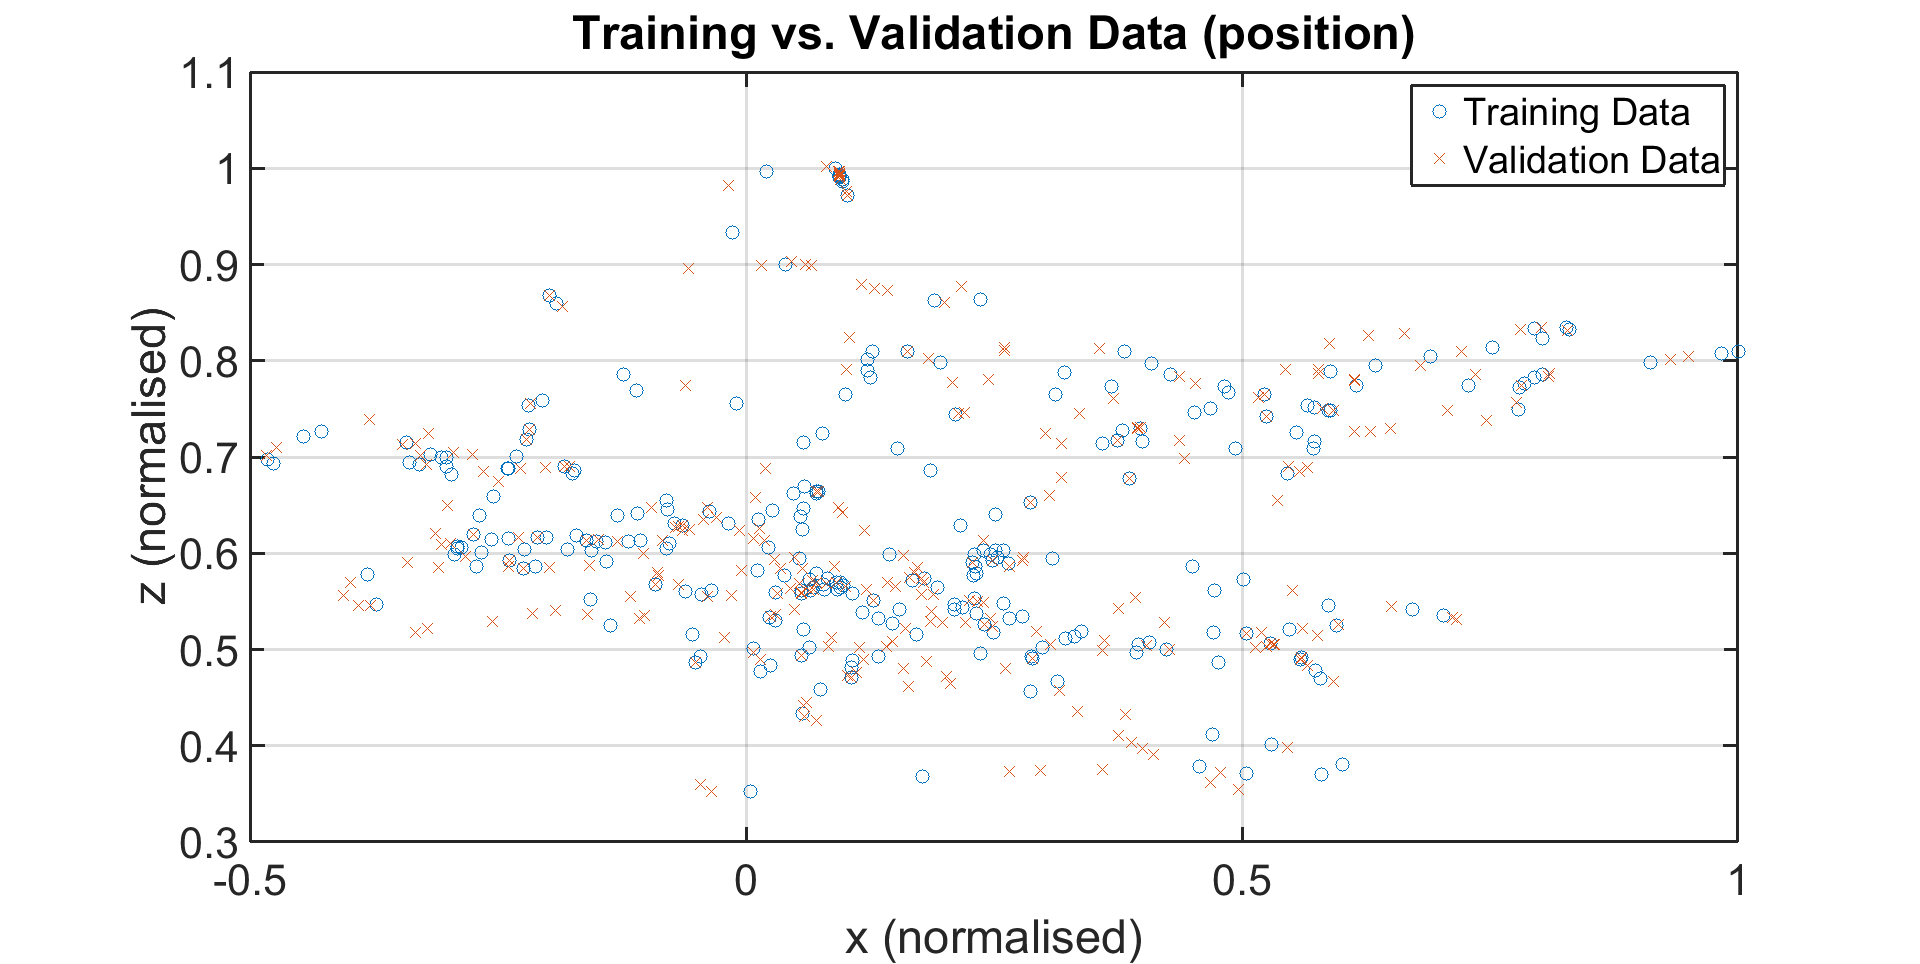
\includegraphics[clip, trim = 80 0 80 0, width=\textwidth]{figures/chapter4/tr_v_v_xz}
    \end{subfigure}
    \caption{}
  \end{subfigure}
  ~
  \begin{subfigure}{\textwidth}
    \begin{subfigure}{0.48\textwidth}
      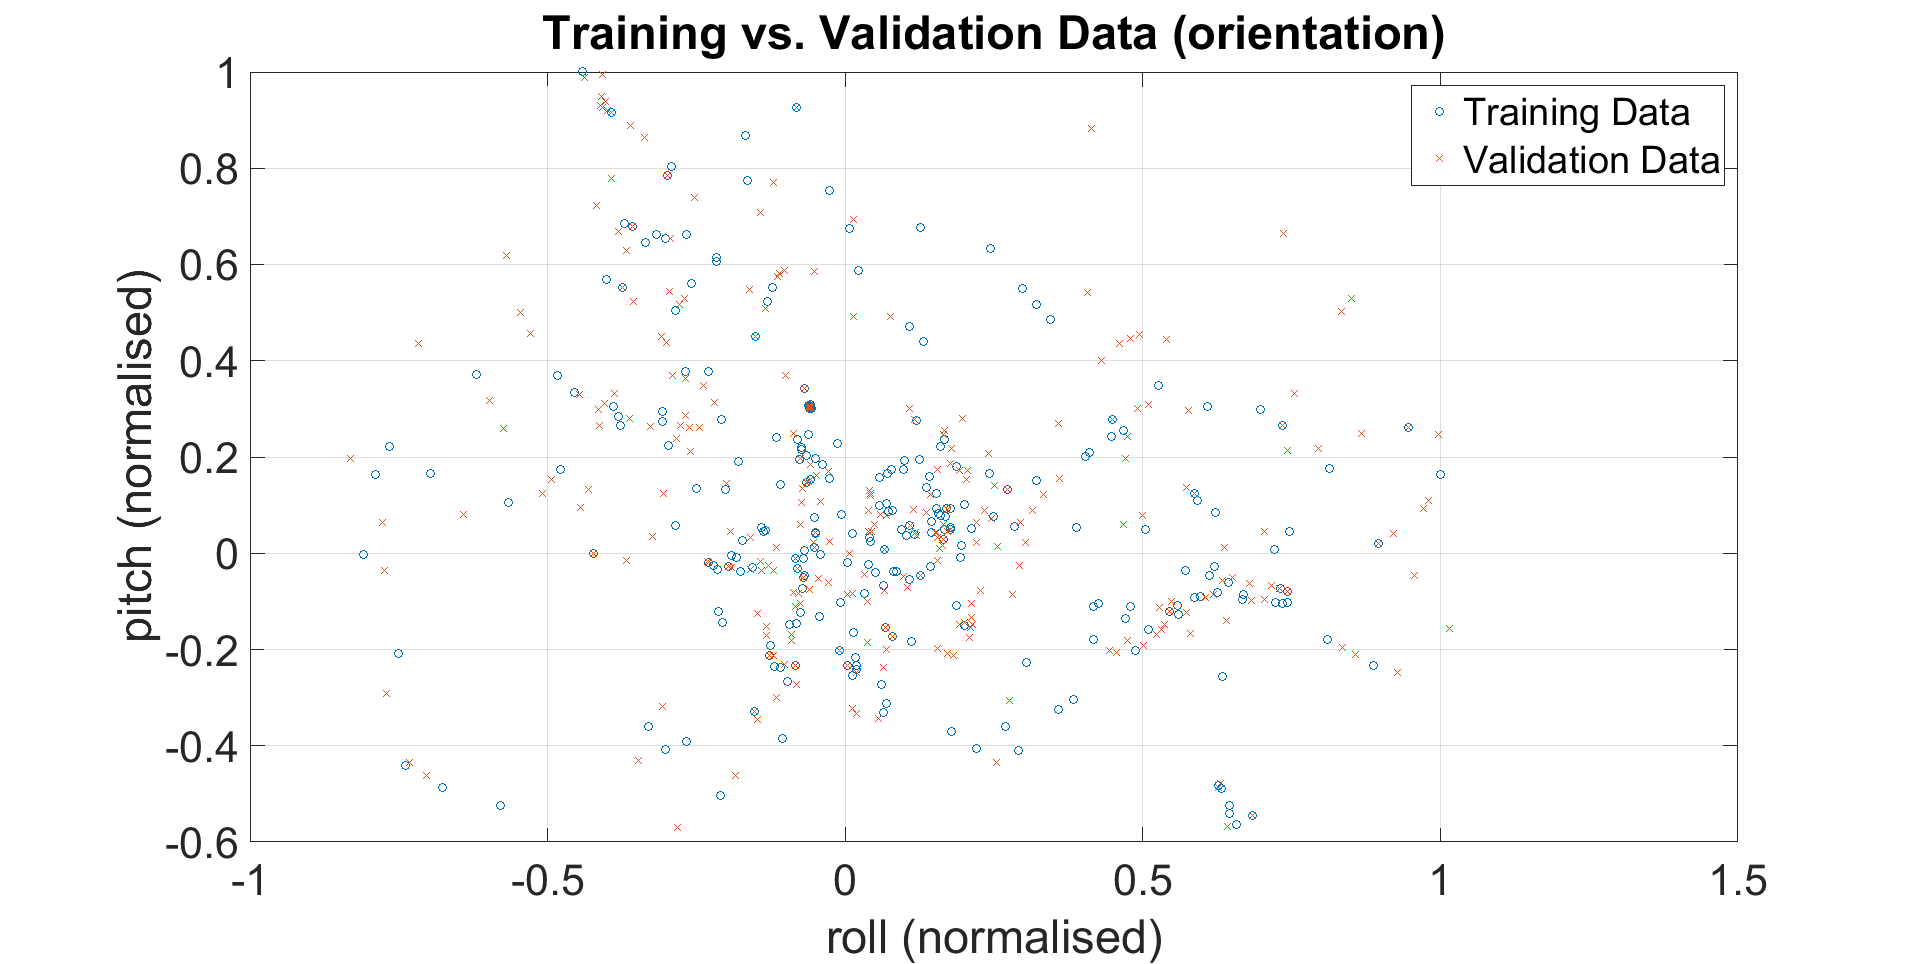
\includegraphics[clip, trim = 80 0 80 0, width=\textwidth]{figures/chapter4/tr_v_v_rollpitch}
    \end{subfigure}
    \begin{subfigure}{0.48\textwidth}
      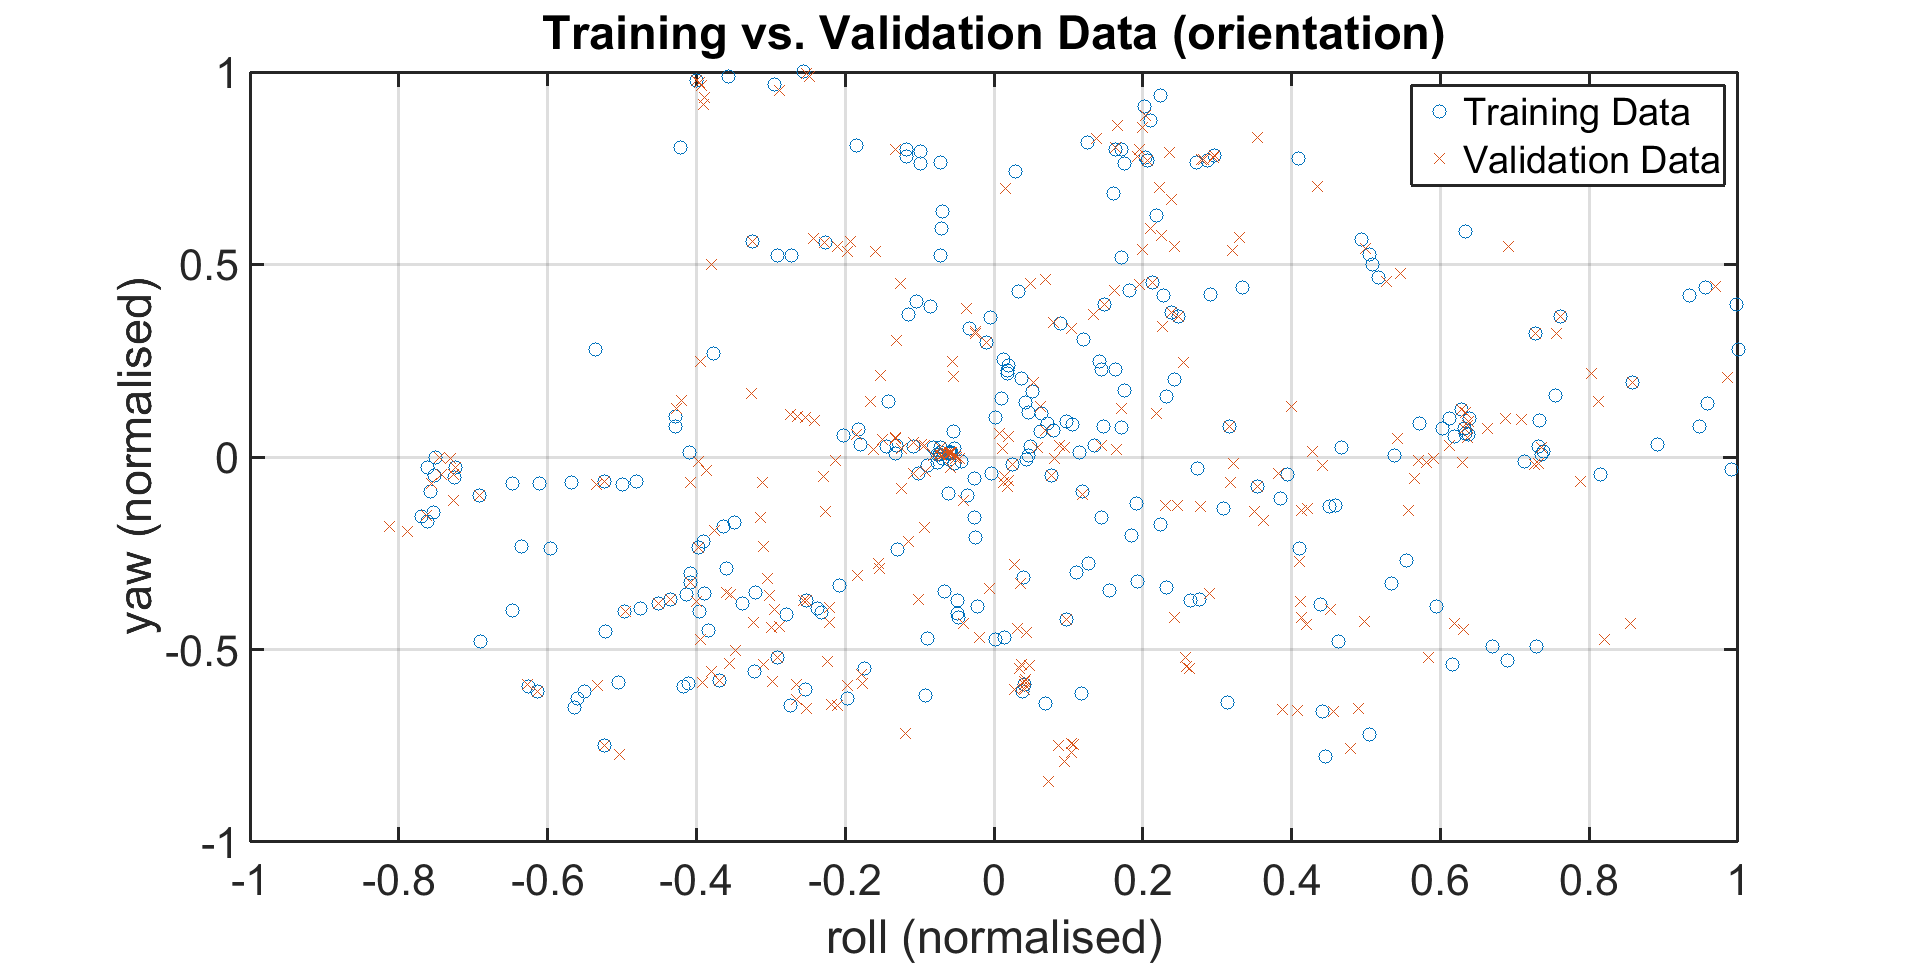
\includegraphics[clip, trim = 80 0 80 0, width=\textwidth]{figures/chapter4/tr_v_v_rollyaw}
    \end{subfigure}
    \caption{}
  \end{subfigure}
  \caption[Scatter plots of the training and validation data. ]{Normalised scatter plots of the translation and rotation data points for the training and validation data sets. Note that the two data sets overlap. This is done on purpose to ensure that the RBFNN does not extrapolate values when the validation set is used as input. }
  \label{fig:chap4-scatter-tr-v}
\end{figure*}

The measurement error was determined by feeding the validation input data into the trained networks and comparing their outputs with the validation error data. The MSEs between the networks' output and validation data were used as measures of accuracy. The validation set was used to tune the \emph{spread} and $\mathit{MN}$ training parameters, where the best combination would produce the smallest training and validation MSEs. 

\section{Results}

With the training and validation data sets selected, network design could begin. Different combinations of training parameters for both networks were tested. It was found that the \emph{spread} parameter had the largest influence over the networks' MSEs during training and validation. This may be because the input data (the orientation in particular) changes relatively quickly and contains a fair amount of noise. It was found that forcing the RBFNN to go through all the points caused the MSE to rise in both networks when they were tested with the validation set, indicating that the networks were being overfitted. It was therefore decided to keep the \emph{spread} parameter relatively small to allow the RBFNNs to ignore what they classify as outlier data and rather describe the general trend within the data. 

Furthermore, changing the maximum number of hidden nodes also influenced the accuracy of the networks. Leaving the $\mathit{MN}$ parameter to its default value will let the maximum number of hidden nodes go up to the number of training samples (300 nodes in this case), making the networks overly complex and slow. It was found that the networks are more accurate with both the training and validation data sets when the hidden nodes number between 20~\% and 30~\% the number of training samples. 

A training parameter combination that was found to work well for the translation network was a \emph{spread} of 8\e{-1} with 85 hidden nodes. This combination gives a normalised MSE of approximately 7.14\e{-2} with the validation data set and 9.44\e{-2} with the training set. For the orientation network it was found that a \emph{spread} of 9\e{-1} with 60 hidden nodes produces good results with a training MSE of 5.13\e{-3} and a validation MSE of 6.1\e{-3}. Leaving the networks to use their default parameter values (1 and 300 respectively) produced a validation MSE 8 orders of magnitude larger than the training MSE\@. This displays the effect of overfitting well. 

Figure~\ref{fig:chap4-rbf-train} show results of the RBFNNs when tested with the training data set. It can be seen that the networks' estimates very closely resemble the training set's error, indicating that the networks are well-trained. 

\begin{figure*}
  \begin{subfigure}{0.48\textwidth}
    \begin{subfigure}{\textwidth}
      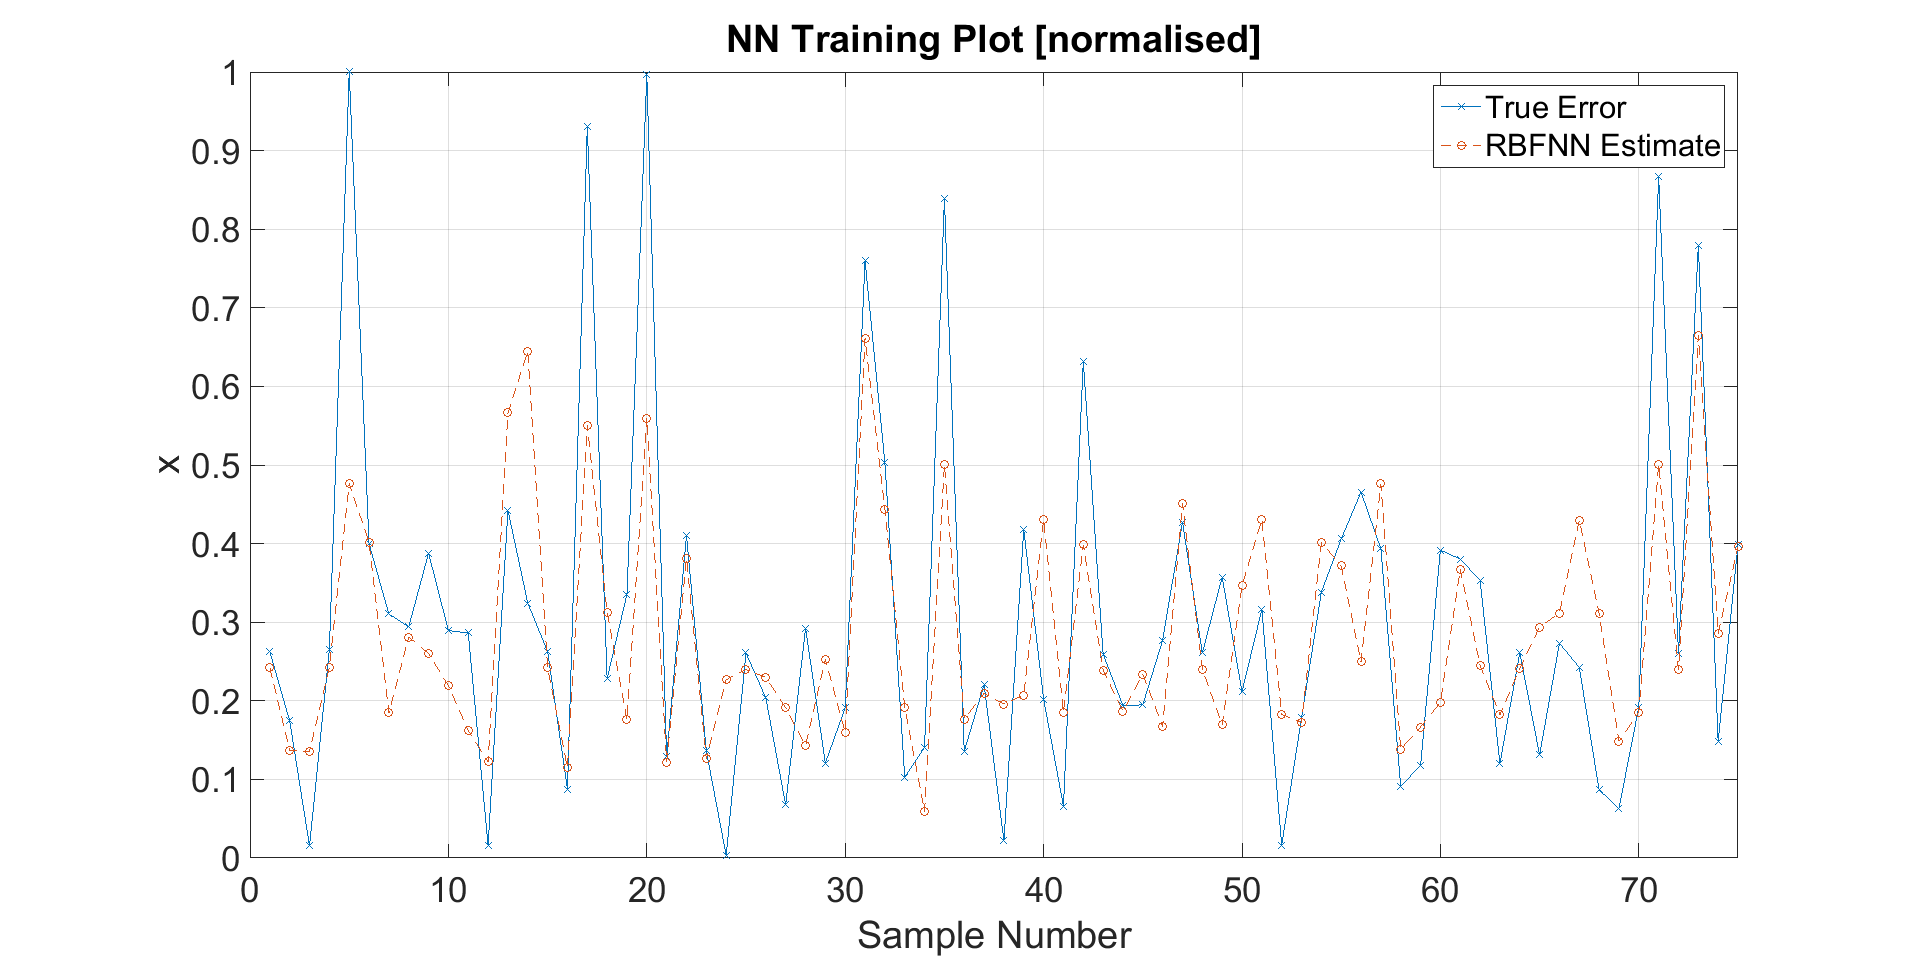
\includegraphics[clip, trim = 80 0 100 0, width=\textwidth]{figures/chapter4/tr_x}
    \end{subfigure}
    \begin{subfigure}{\textwidth}
      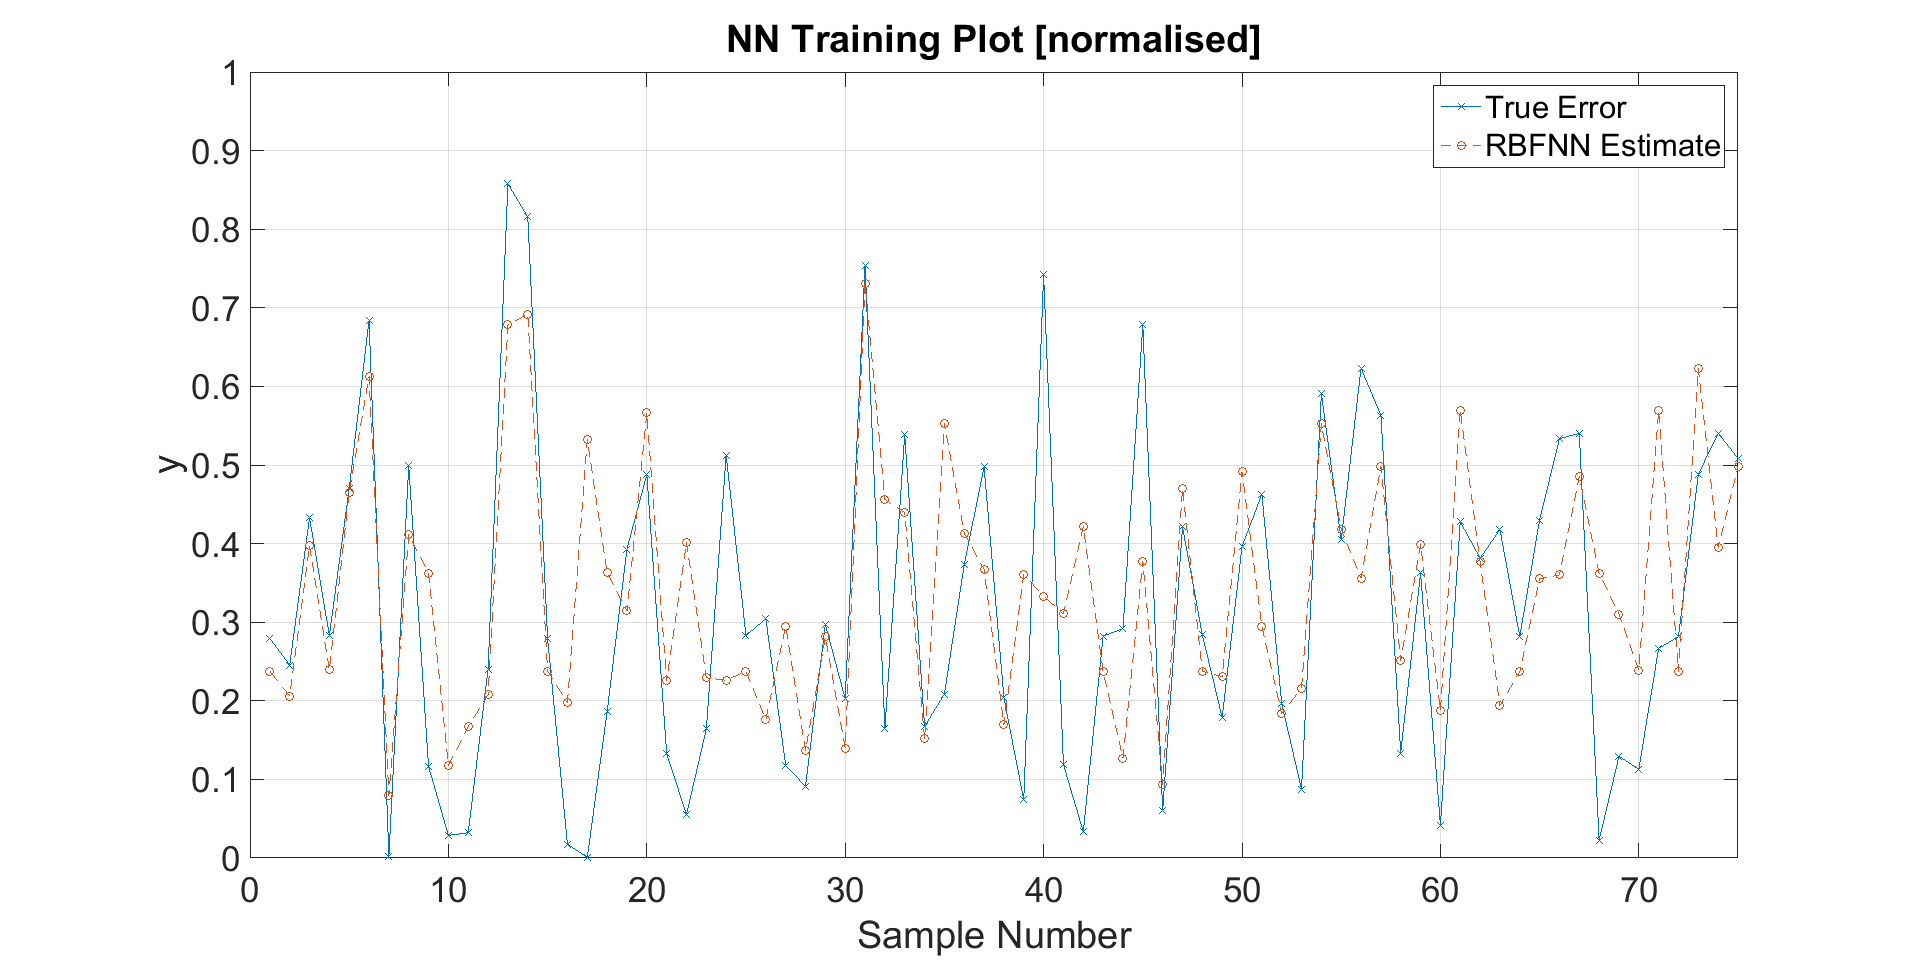
\includegraphics[clip, trim = 80 0 100 0, width=\textwidth]{figures/chapter4/tr_y}
    \end{subfigure}
    \begin{subfigure}{\textwidth}
      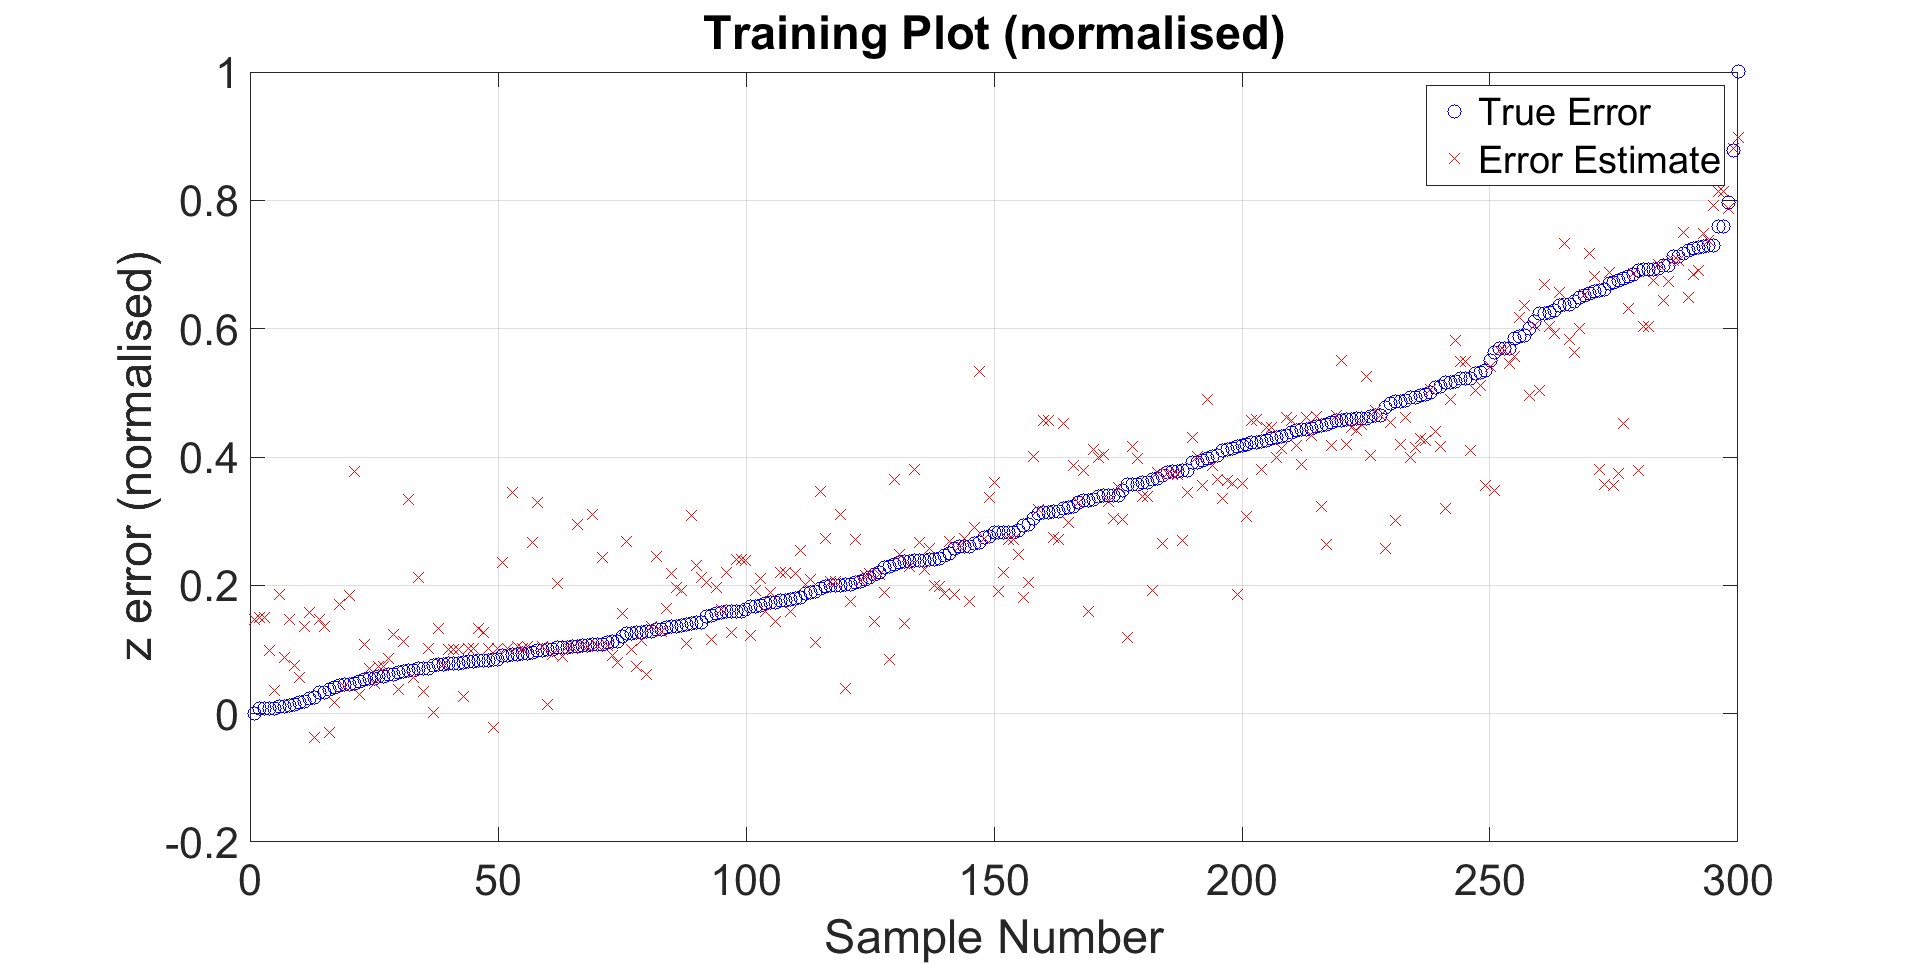
\includegraphics[clip, trim = 80 0 100 0, width=\textwidth]{figures/chapter4/tr_z}
    \end{subfigure}
    \caption{}
  \end{subfigure}
  \begin{subfigure}{0.48\textwidth}
    \begin{subfigure}{\textwidth}
      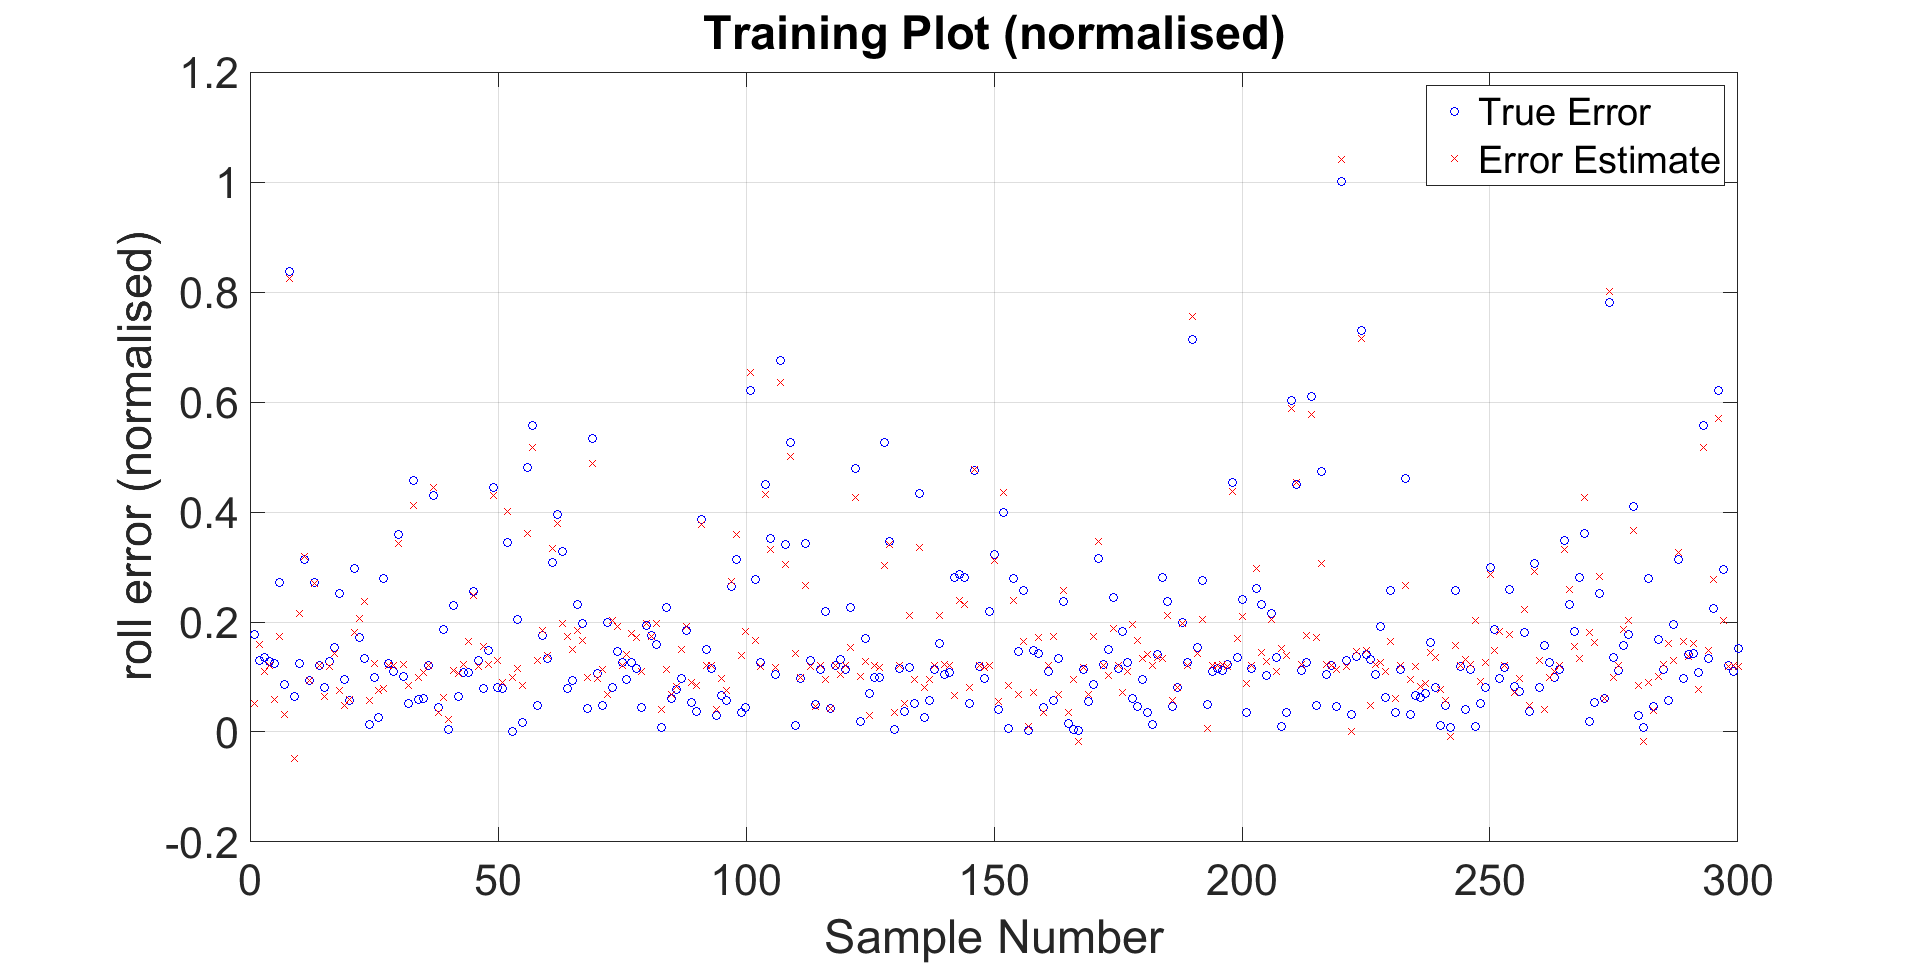
\includegraphics[clip, trim = 80 0 100 0, width=\textwidth]{figures/chapter4/tr_roll}
    \end{subfigure}
    \begin{subfigure}{\textwidth}
      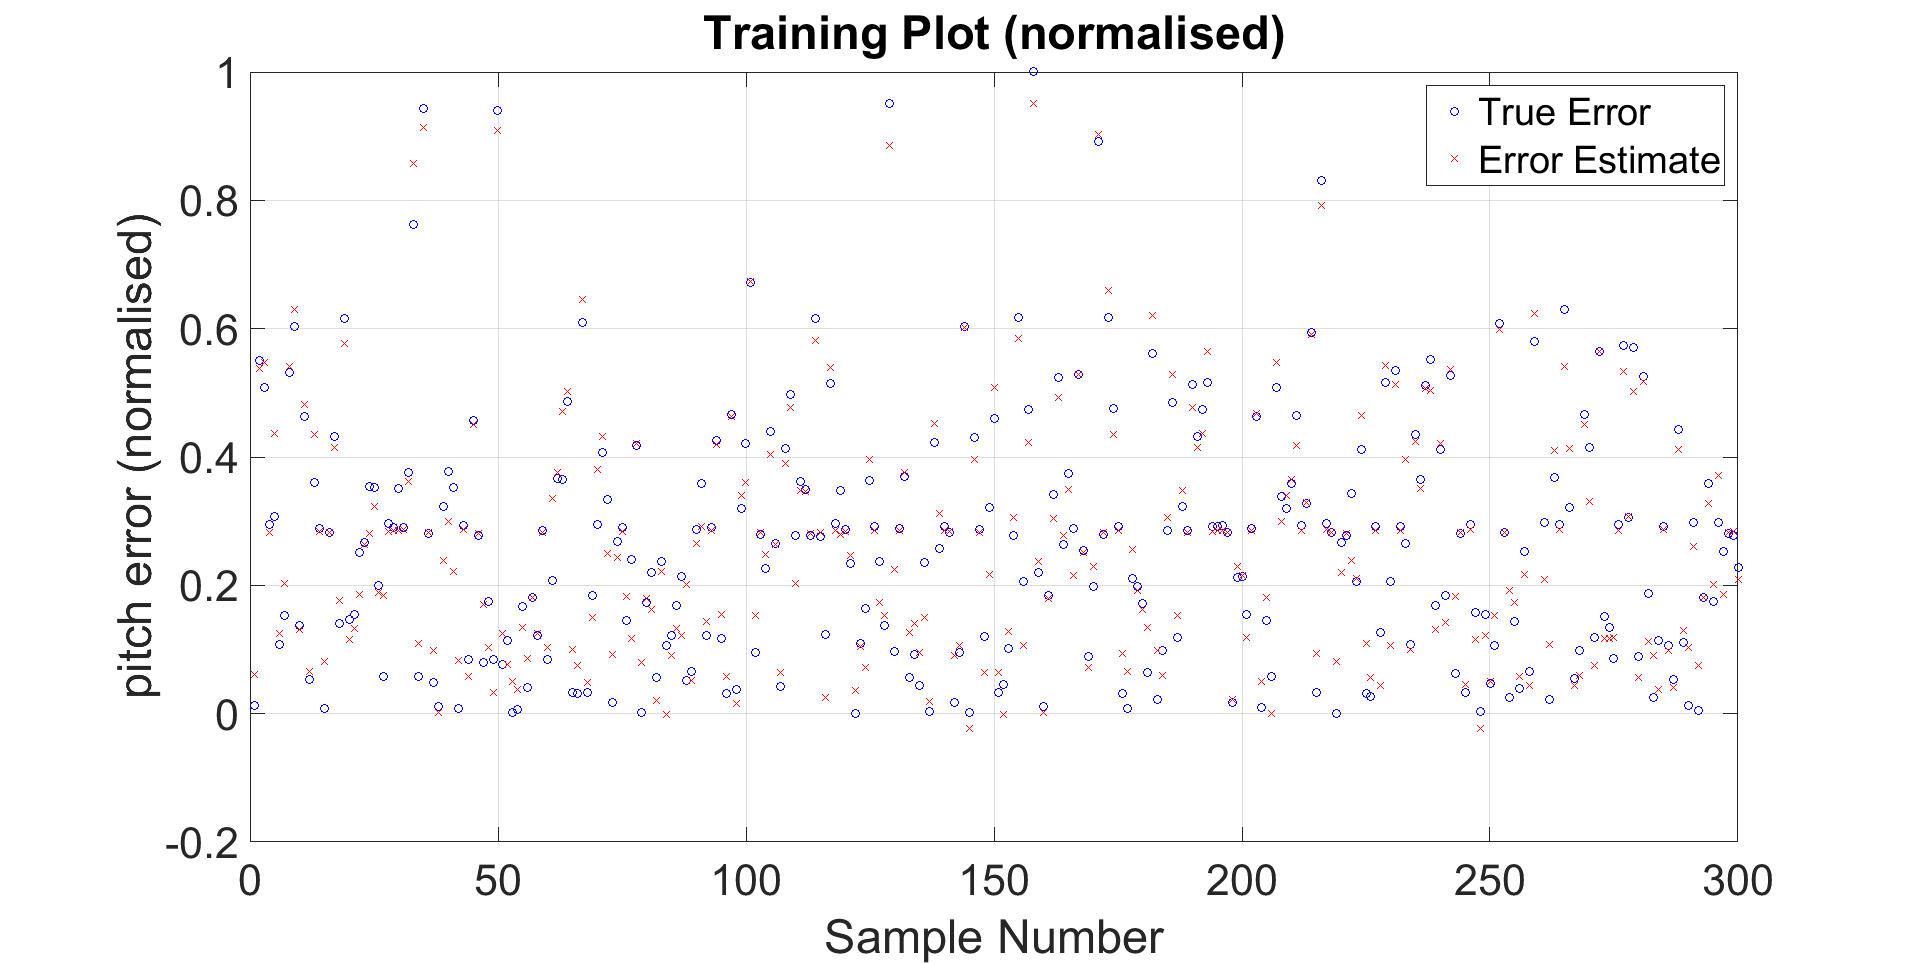
\includegraphics[clip, trim = 80 0 100 0, width=\textwidth]{figures/chapter4/tr_pitch}
    \end{subfigure}
    \begin{subfigure}{\textwidth}
      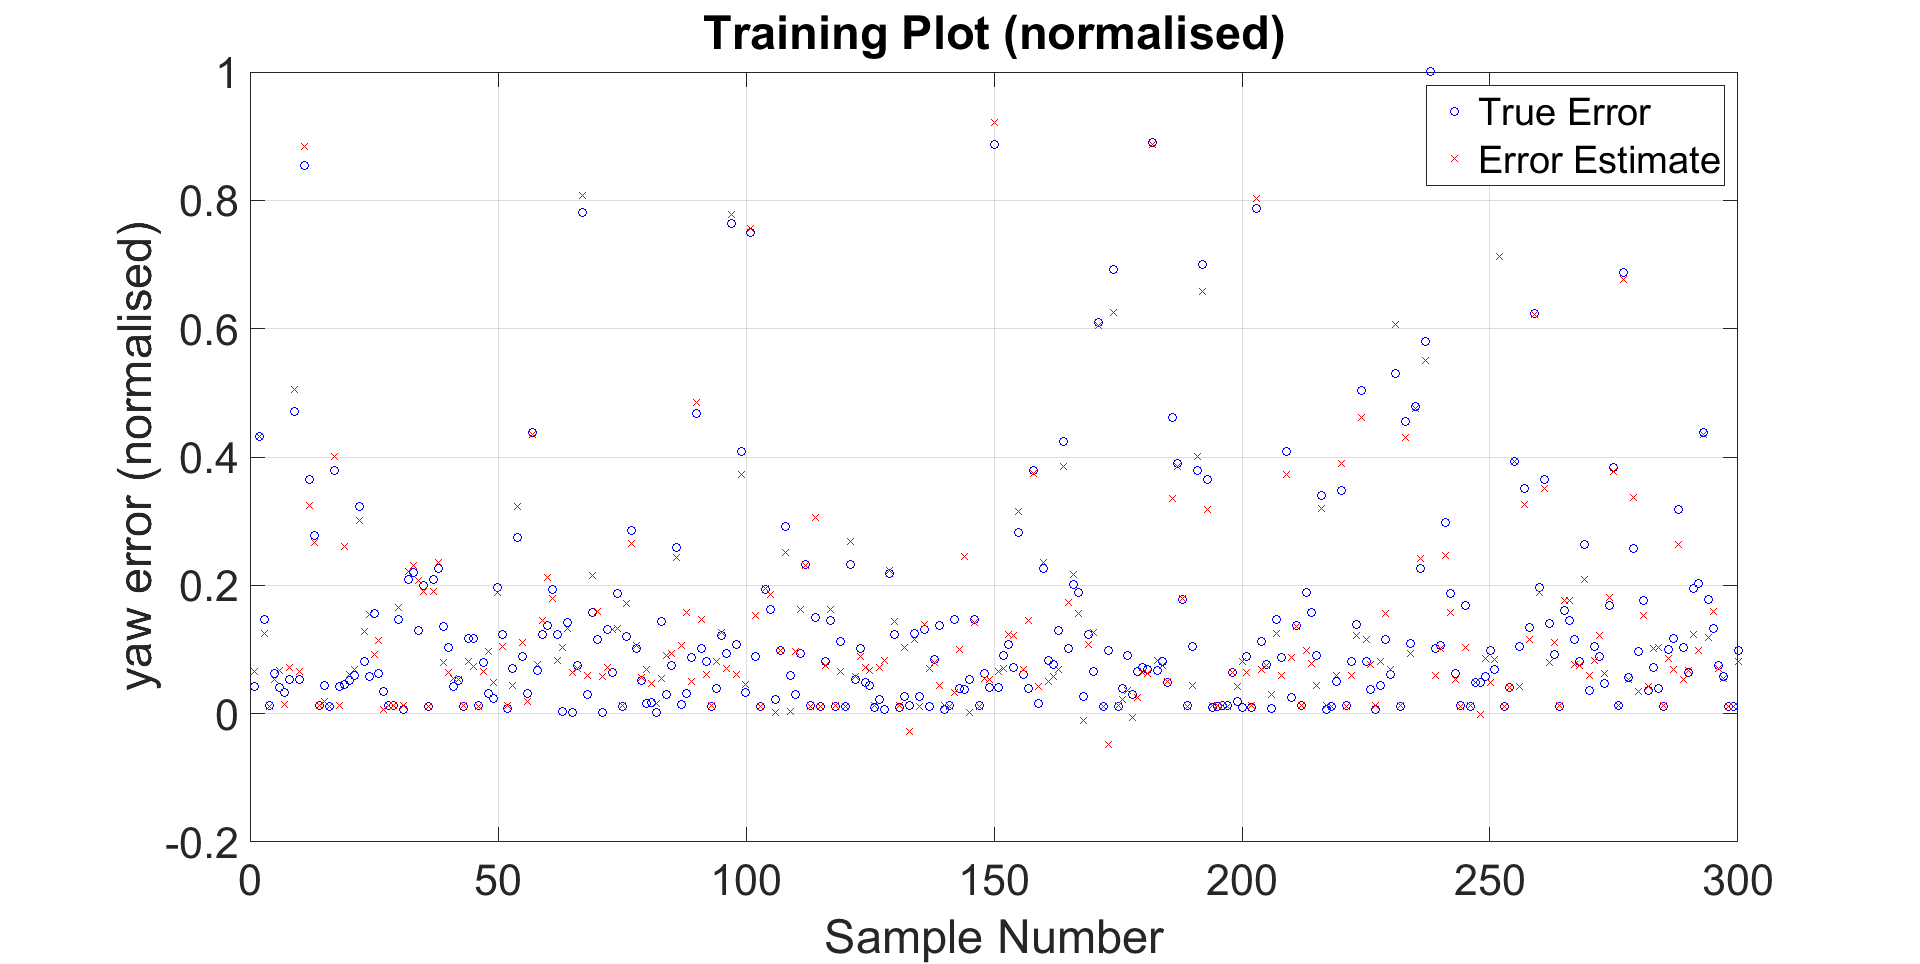
\includegraphics[clip, trim = 80 0 100 0, width=\textwidth]{figures/chapter4/tr_yaw}
    \end{subfigure}
    \caption{}
  \end{subfigure}
  \caption[The output of the RBFNN when used with the training set input.]{Plots of the output of the RBFNN for the different dimensions when used with the training data set.}
  \label{fig:chap4-rbf-train}
\end{figure*}

Figure~\ref{fig:chap4-rbf-valid} shows the networks' output when tested with the validation data set. Here it can be seen that the RBFNNs' error estimates very closely resemble the true error, with the position MSE being smaller in the validation case than for the training case. 

\begin{figure*}
  \begin{subfigure}{0.48\textwidth}
    \begin{subfigure}{\textwidth}
      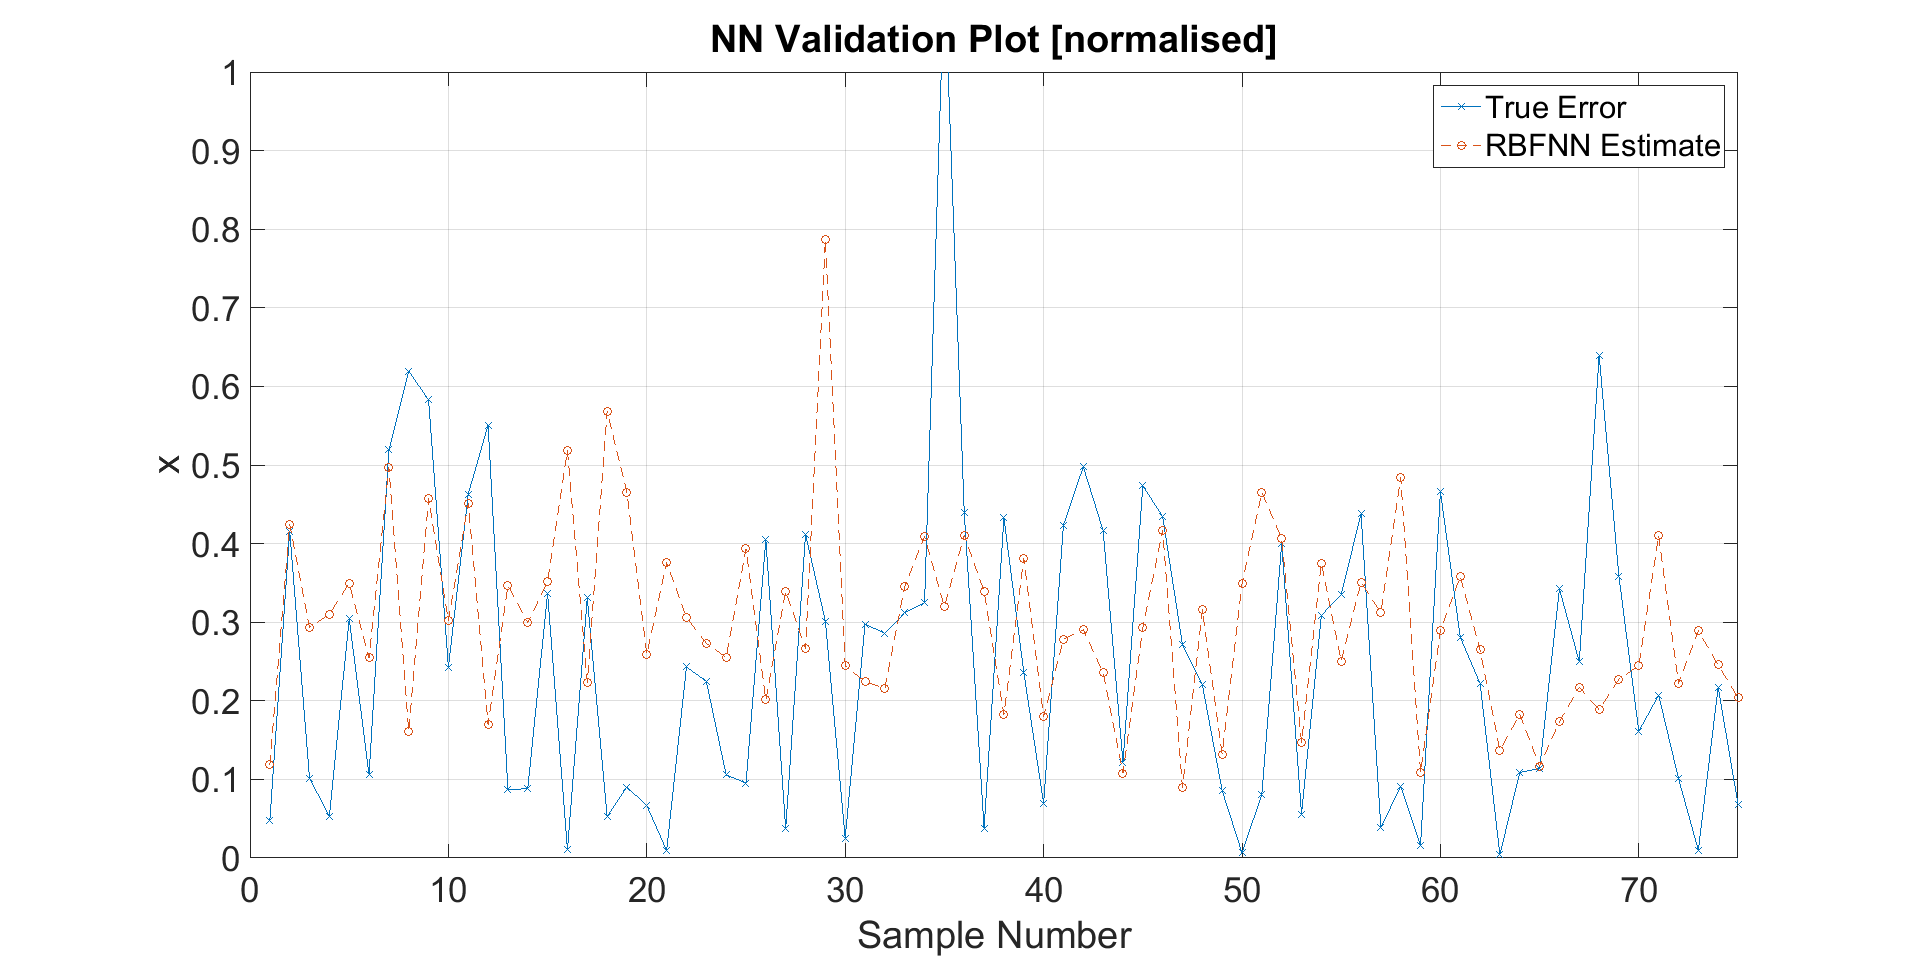
\includegraphics[clip, trim = 80 0 100 0, width=\textwidth]{figures/chapter4/v_x}
    \end{subfigure}
    \begin{subfigure}{\textwidth}
      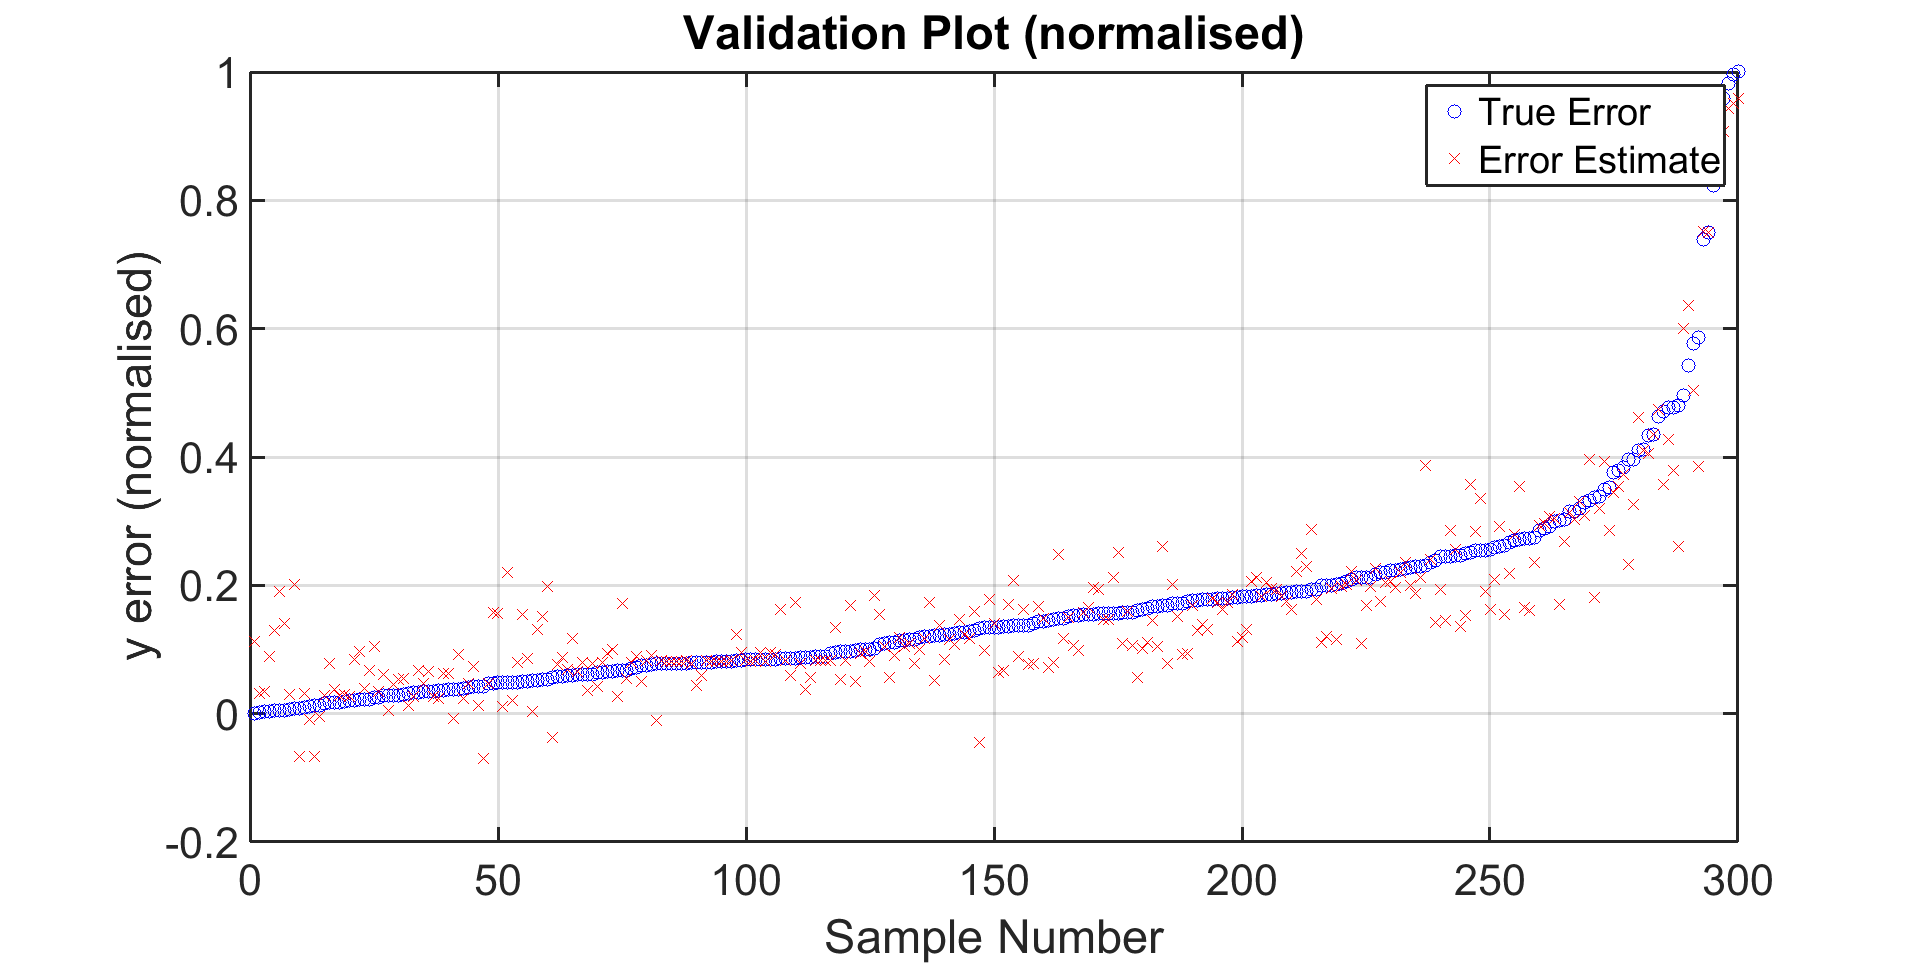
\includegraphics[clip, trim = 80 0 100 0, width=\textwidth]{figures/chapter4/v_y}
    \end{subfigure}
    \begin{subfigure}{\textwidth}
      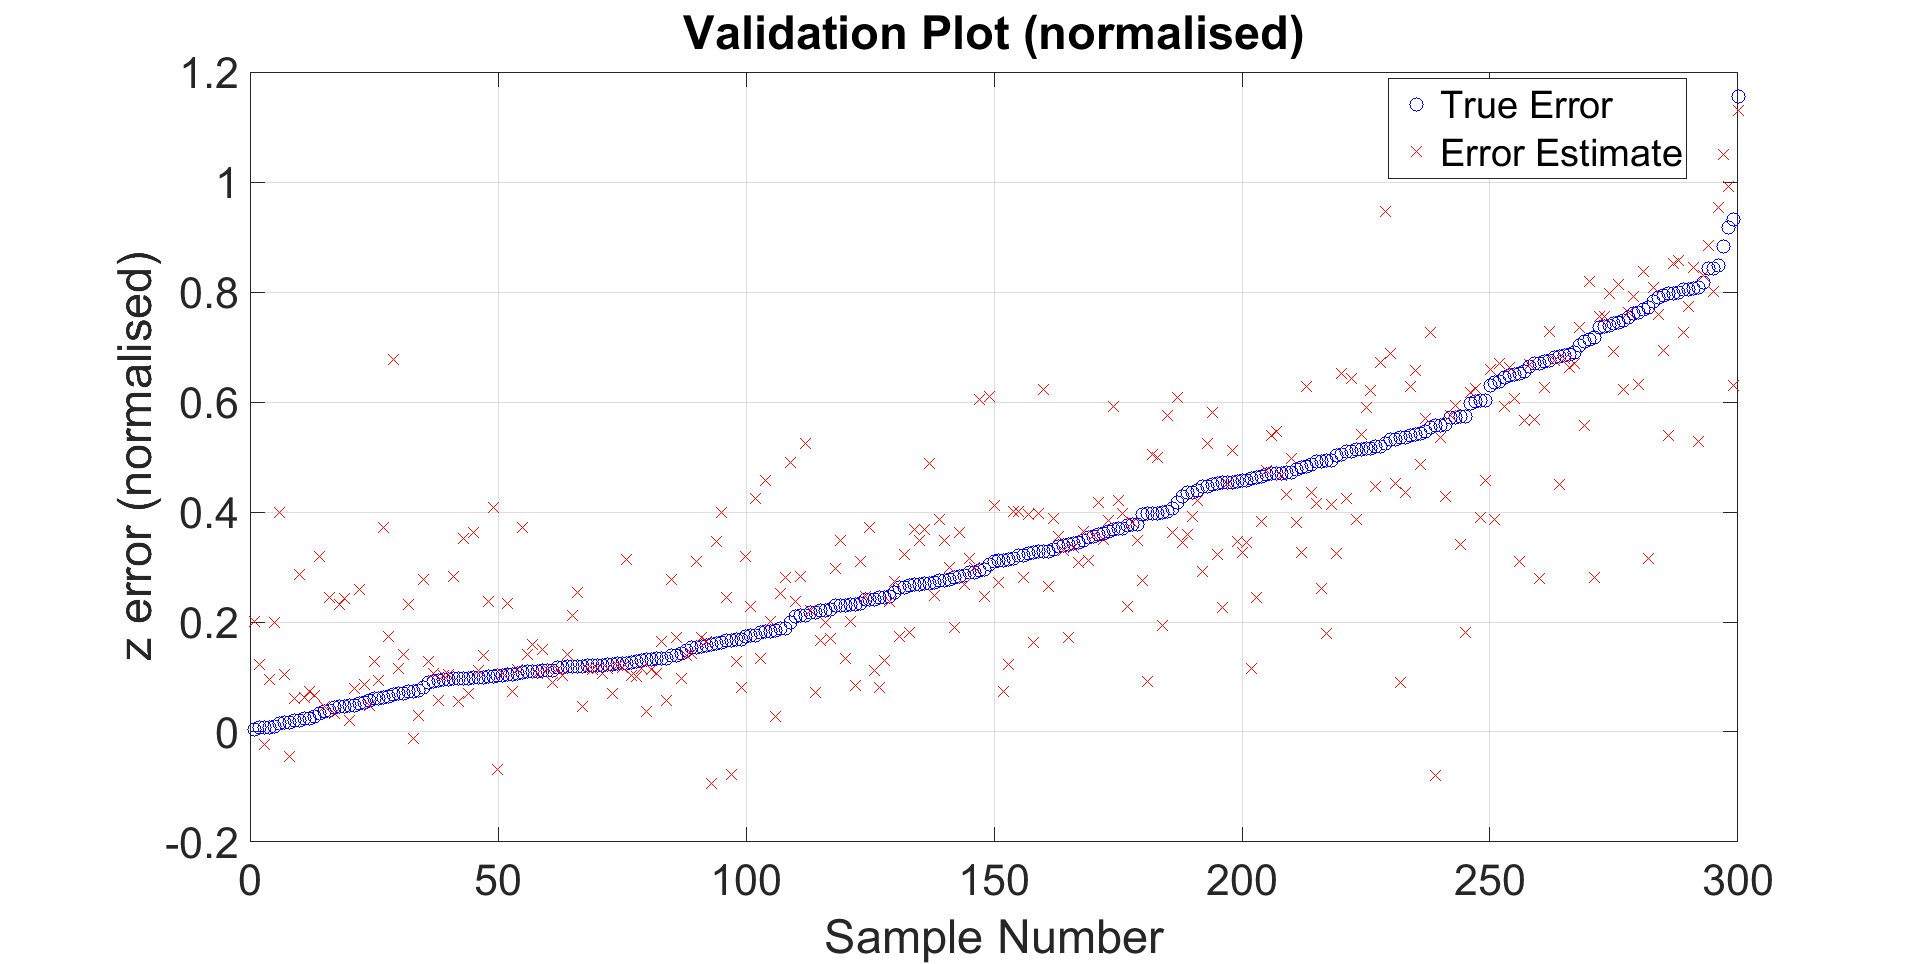
\includegraphics[clip, trim = 80 0 100 0, width=\textwidth]{figures/chapter4/v_z}
    \end{subfigure}
    \caption{}
  \end{subfigure}
  \begin{subfigure}{0.48\textwidth}
    \begin{subfigure}{\textwidth}
      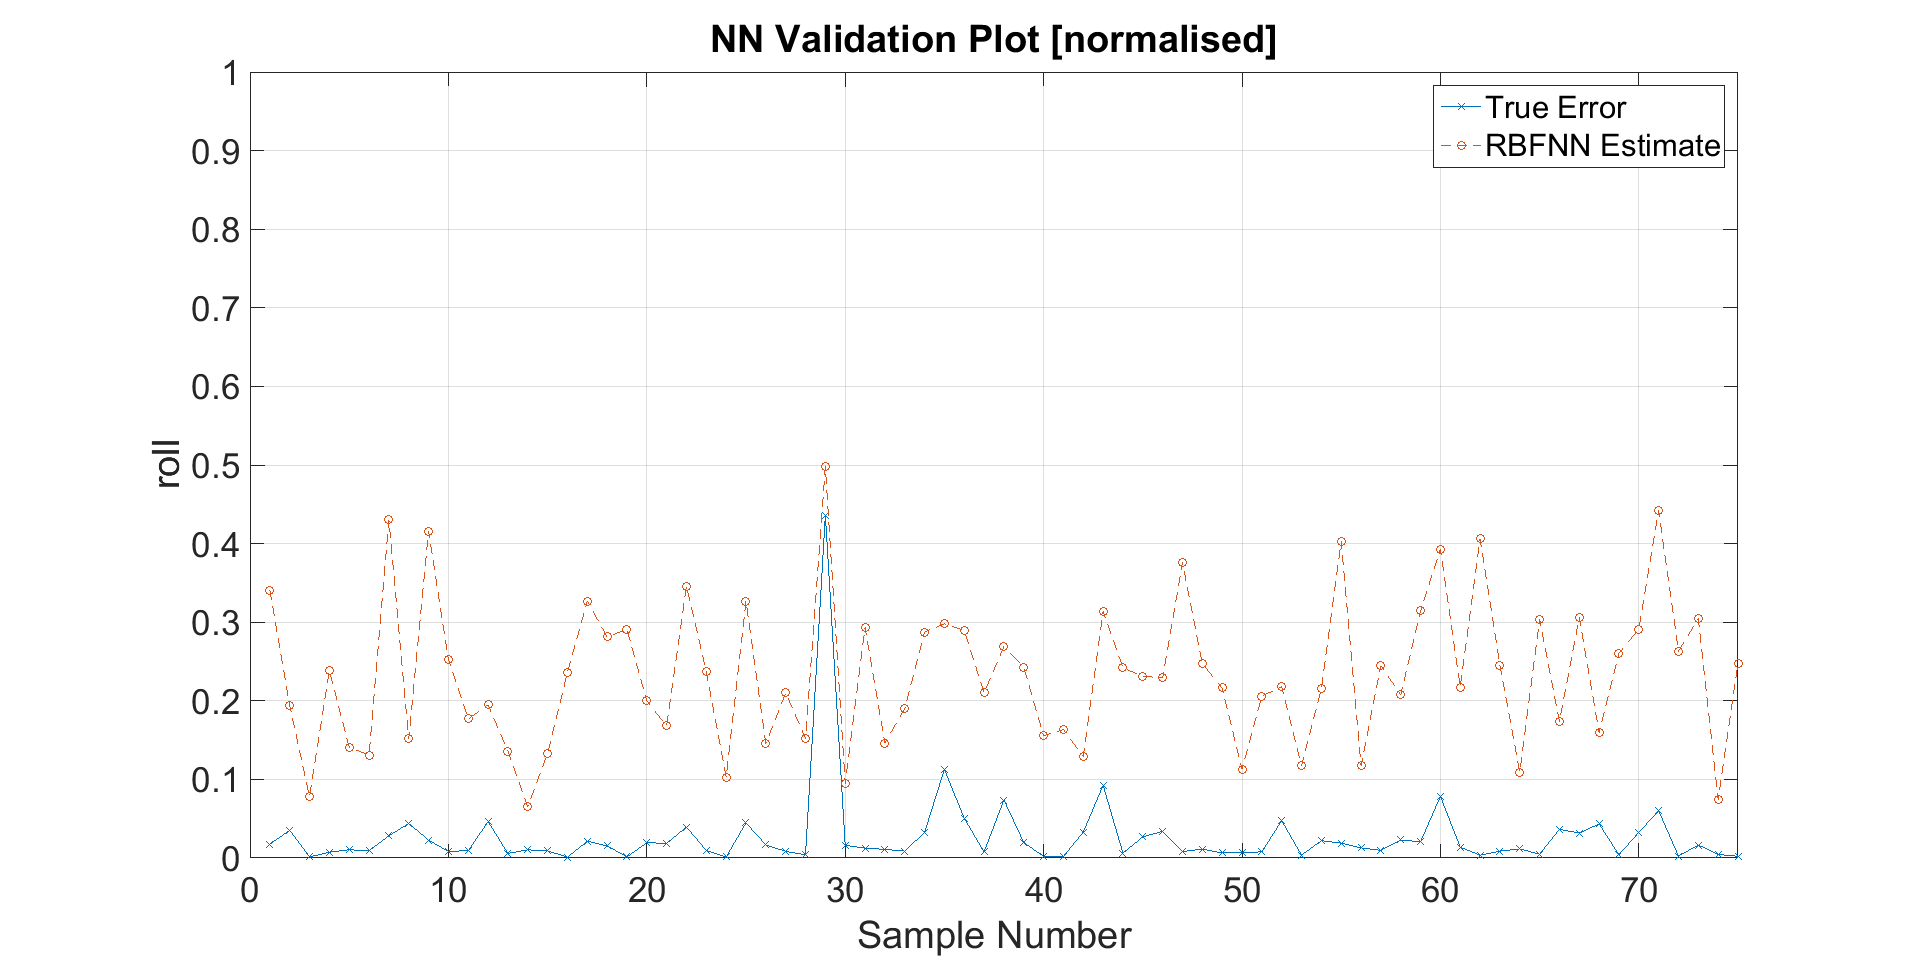
\includegraphics[clip, trim = 80 0 100 0, width=\textwidth]{figures/chapter4/v_roll}
    \end{subfigure}
    \begin{subfigure}{\textwidth}
      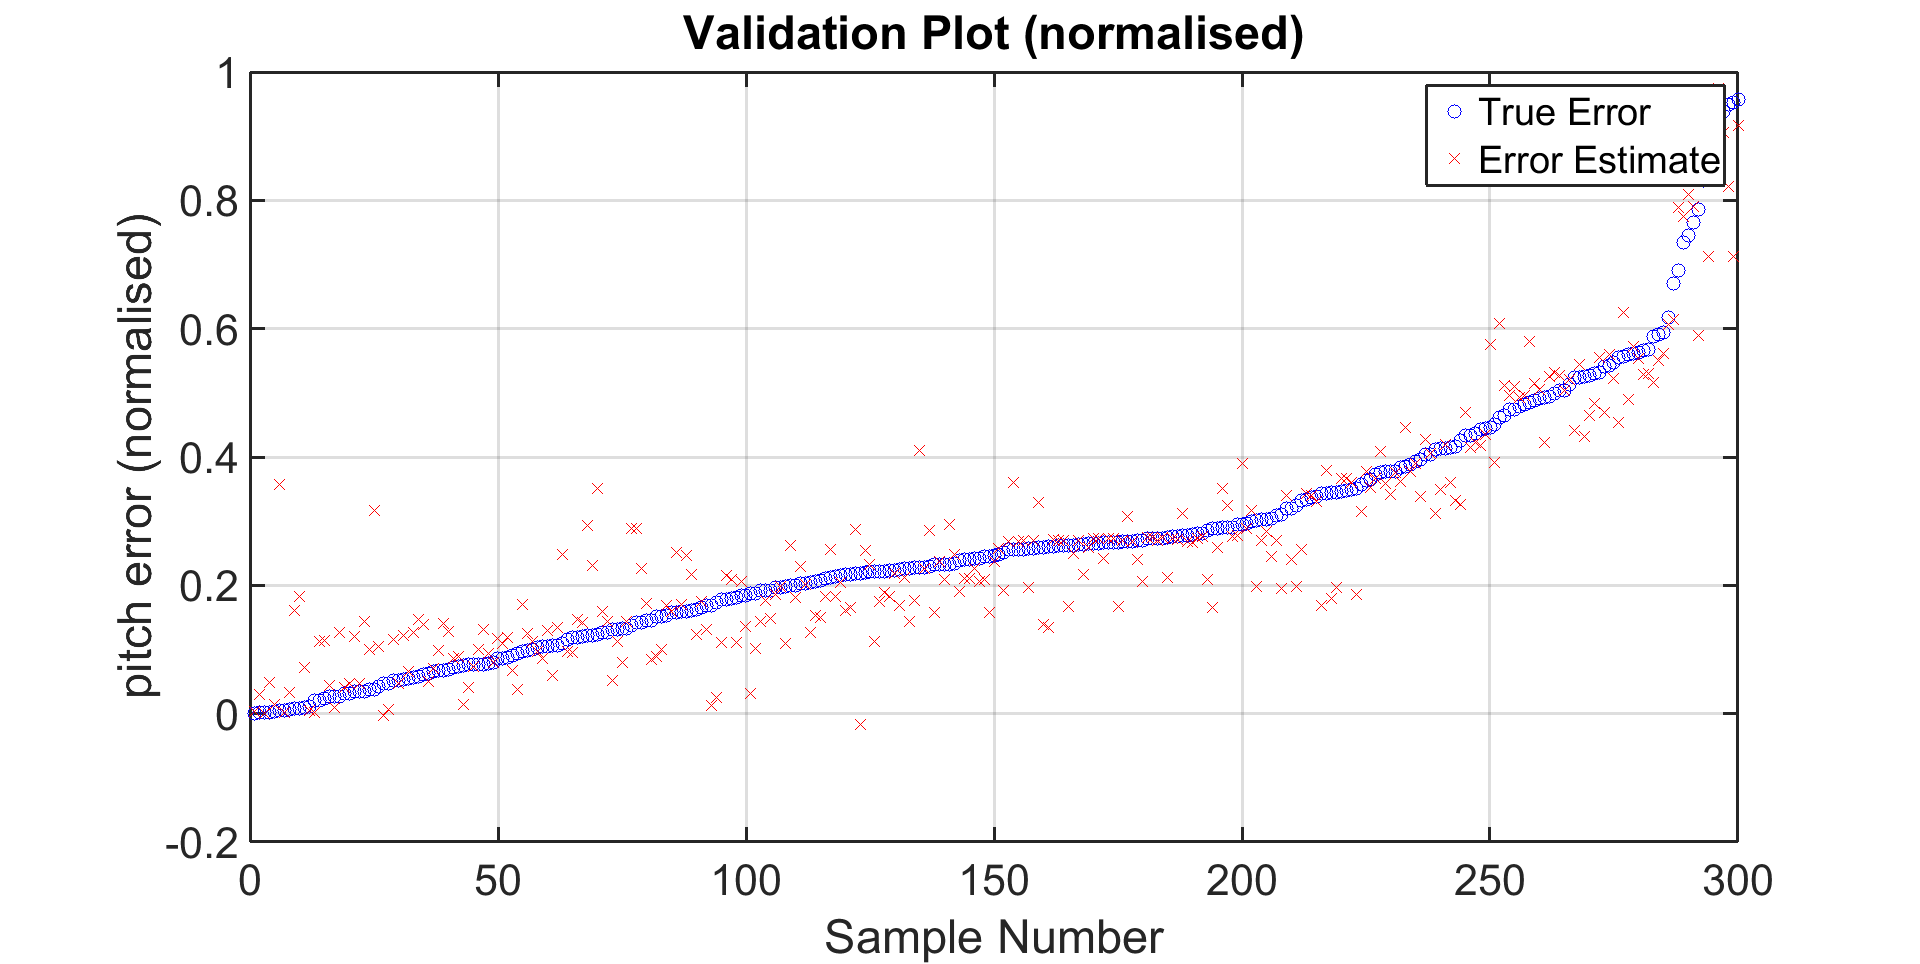
\includegraphics[clip, trim = 80 0 100 0, width=\textwidth]{figures/chapter4/v_pitch}
    \end{subfigure}
    \begin{subfigure}{\textwidth}
      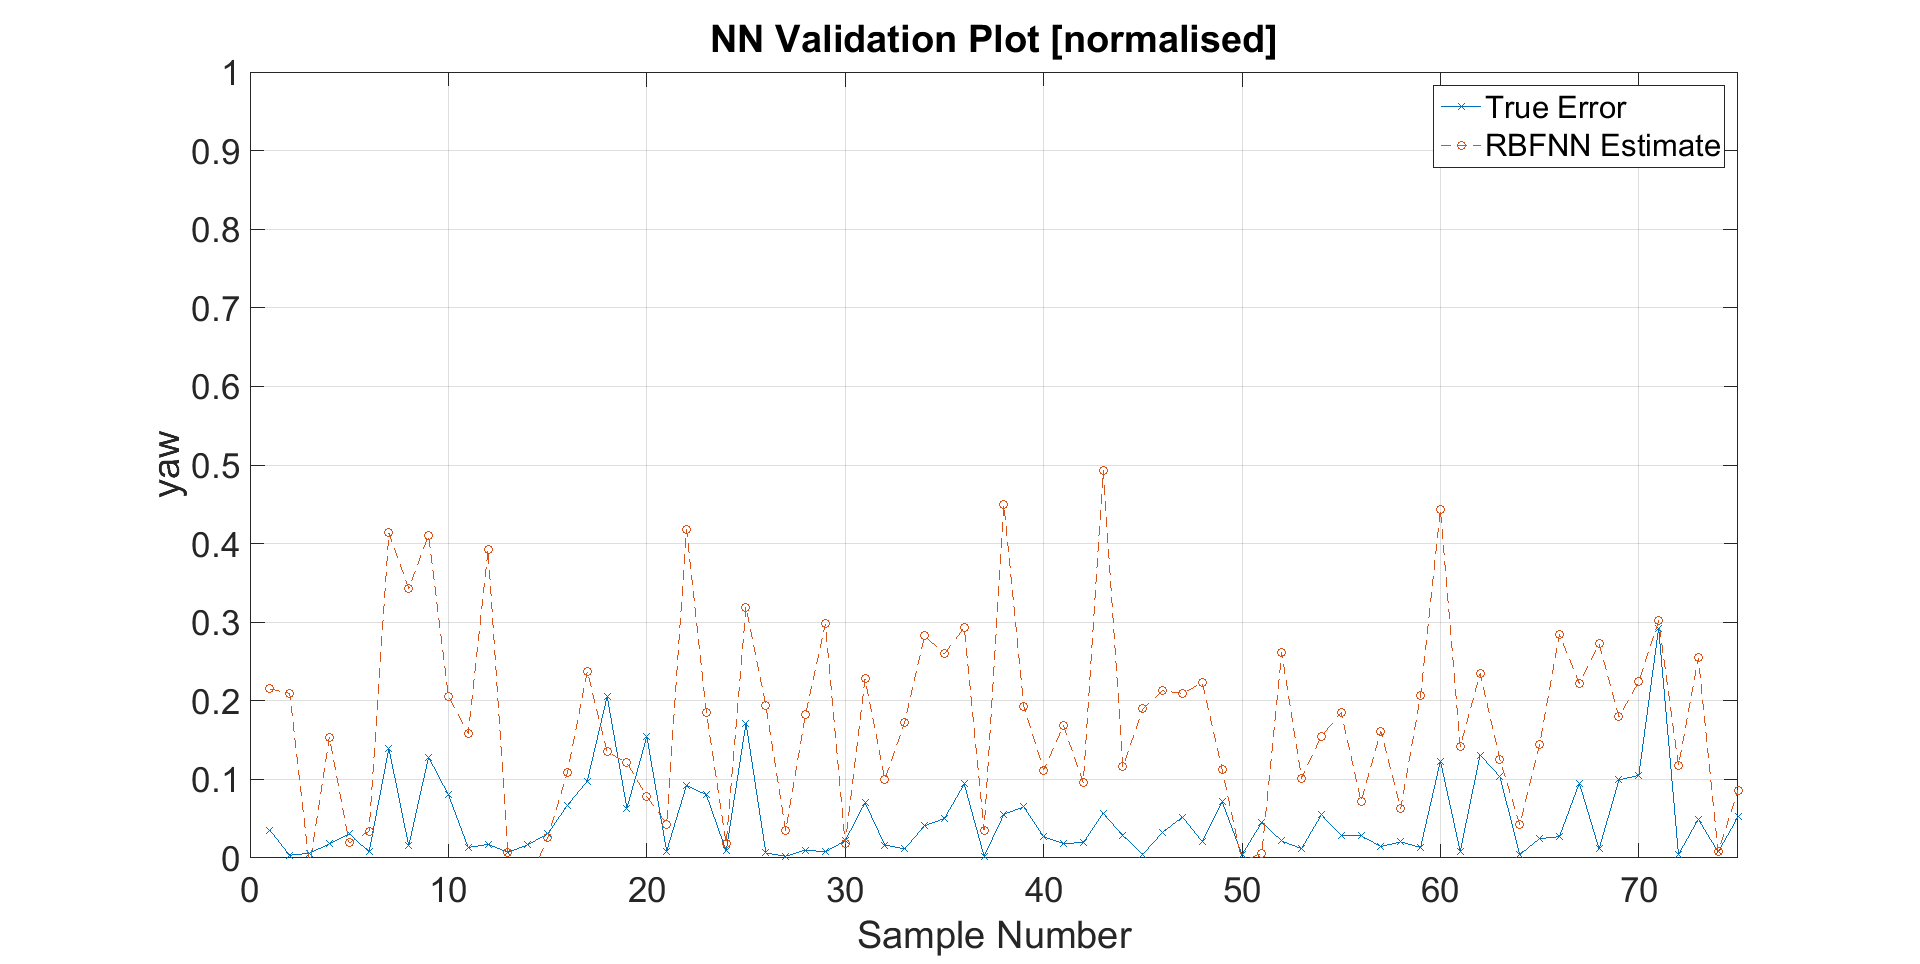
\includegraphics[clip, trim = 80 0 100 0, width=\textwidth]{figures/chapter4/v_yaw}
    \end{subfigure}
    \caption{}
  \end{subfigure}
  \caption[The output of the RBFNN with the validation set input.]{Plots of the output for the different dimensions of the RBFNN when used with the validation data set.}
  \label{fig:chap4-rbf-valid}
\end{figure*}

These plots show that the networks are well trained and produce accurate estimates of both the training and validation data sets. 
\section{Conclusion}

In this chapter two neural networks were designed to model and predict the complex and dimensionally dependant pose measurement error of the CVS.\@ A radial basis function neural network was selected to do this: the networks take a six-dimensional pose measurement vector from the CVS and outputs the corresponding measurement error for the input sample. The network was trained and validated by two different data sets from the same measurement test and produce a validation mean square error of 7.14\e{-2} 6.1\e{-3} for the position and orientation network respectively, indicating a good model fit for the data. 

The trained networks are now ready to predict the measurement error for the CVS with pose measurement data generated by a quadcopter in flight. This data can then be used to determine the pose estimation accuracy of a quadcopter in flight. 
